\PassOptionsToPackage{quiet}{xeCJK}
\documentclass{beaulivre}

%\usepackage{multicol}
\usepackage{booktabs}
\usepackage{tikz}
\usepackage{pgfplots}
\usepackage{cancel}
\usepackage{caption}
\usepackage{makeidx}
\usepackage{geometry}
\usepackage{sidenotes}
\usepackage{amsmath}
\usepackage{amssymb}
\usepackage{hyperref}
\usepackage{cuted}
\usepackage{amsthm}
\usepackage{ulem}
\usepackage{graphicx}
\geometry{a4paper}

\bibliographystyle{alpha}

\title{我的考研数学笔记}
\author{王世鑫\thanks{E-mail:w2683107566@live.com}}
\date{\today}

\begin{document}

%\maketitle

\begin{figure}[h]
    \centering
    \includegraphics[width=2cm]{cc-icon.png} 
\end{figure}

\frontmatter
在科学上面没有平坦的大道,只有不畏劳苦沿着陡峭的山路攀登的人,才有希望达以光辉的顶点。

这是我第一次正式使用 \LaTeX{} 来进行写作。作为我的考研数学复习的笔记之用。
作笔记本身是对知识的一种复盘和总结,使用 \LaTeX{} 可以对这个过程增添几分乐趣。
某种程度上能和我同期正在缓慢进行的个人C++项目 koios 一样,在枯燥乏味的考研备考生活中增添几分色彩。

这本笔记将会收录一些在各类成体系的考研教学视频以及和考研数学相关的文章、
视频中提到的做题方法和一些基本的定理以供本人成查阅。
由于内容是数学相关的内容,本人并非数学专业学生,因此在表述上难免出现令数学人嗤之以鼻的不严谨,
如果您发现了一些这样的现象,欢迎直接提PR对本笔记进行修改,
如果觉得麻烦,也烦请您直接以各种形式告知我,感激不尽。
我会在每周复盘进行笔记的时候对PR进行集中处理。


\tableofcontents

\mainmatter
\twocolumn
\chapter{全局通用技术}

\begin{lemma}
\begin{multline*}
	f, g \mbox{在} x_0 \mbox{有公共切线} \\ \Rightarrow f(x_0) = g(x_0), f'(x_0) = g'(x_0)
\end{multline*}
\end{lemma}
上述内容中小心遗漏 $f(x_0) = g(x_0)$

\begin{definition}
    \begin{equation}
        \mathbf{C}_{k}^{n}\binom{n}{k} = \frac{n!}{k!(n-k)!}
    \end{equation}
\end{definition}

\begin{lemma}
    \begin{align*}
        (a+b)^3 = a^3 + 3a^2b + 3ab^2 + b^3\\
        (a-b)^3 = a^3 - 3a^2b + 3ab^2 - b^3
    \end{align*}
\end{lemma}

\section{函数}

无论是导数还是积分,相关题目和函数性质(图像、单调性等)相关性总是很大,
在处理的时候要善于利用函数的性质,辅助解题。
利用函数性质辅助解题的有例子:
题目 
\begin{itemize}

    \item   \cite[page 70, pdf 81, 例1]{we} 和 
            \cite[page 75, pdf 86, 例6]{we}利用函数是偶函数,
            因此图像对称,从而你确定第二条渐近线。

    \item   题目 \cite[page 77, pdf 88, 例5, 例6]{we} 
            通过观察函数图像,辅助确定根的个数,
            有关根的个数请参阅 \ref{number-of-roots-question}。

    \item   题目 \cite[page 107, pdf 118, example 4]{we}
            认识到原函数是偶函数,进而简化求值过程。

\end{itemize}

\subsection{如何联系函数和导数}

TODO
%TODO

\section{Tylor Series and Formula} \label{tylor}

\subsection{公式和形式}

\begin{definition}[泰勒公式的一般形式]
	\begin{equation}
		f(x)=\sum_{i=0}^{n}{\frac{f^{(i)}(x_0)}{i!}(x-x_0)^i}+R_n(x)
	\end{equation}
	其中,$f^{(i)}(x_0)$表示$f(x)$在$x_0$处的$i$阶导数,$R_n(x)$表示余项,有多种形式,例如:
	\begin{align*}
		&R_n(x)=\frac{f^{(n+1)}(\xi)}{(n+1)!}(x-x_0)^{n+1}, \\ &\xi \in [x,x_0]\ or \ \xi \in [x_0,x]
	\end{align*}
\end{definition}

In summary, the Peano remainder focuses on 
the local behavior of the function near the point of expansion 
and gives a rough upper bound on the error for a specific value of $x$. 
\begin{definition}{The Cauchy remainder}
    \[
        R_n=\dfrac{(x-x^*)^n}{n!}(x-x_0)f^{(n+1)}(x^*)
    \]
    where $x^*$ is in $[x_0,x]$ (Hamilton 1952).
\end{definition}
The \textbf{Cauchy remainder provides a more global perspective by 
considering the behavior of derivatives across a broader 
interval between $x_0$ and $x$}. It gives a more refined estimate 
of the error over that interval. This distinction in the scope 
of accuracy makes the Cauchy remainder more useful when you want 
to understand how well the Taylor polynomial approximates the function 
across a larger range of values.

下面是常用的一些Tylor公式
\begin{align}
    \label{eq:useful-tylor-expandations}
	\notag e^x&=1+x+\frac{x^2}{2!}+\frac{x^3}{3!} \\ &+\cdots+\frac{x^n}{n!}+o(x^n)\\
	\notag \ln(1+x)&=x-\frac{x^2}{2}+\frac{x^3}{3}\\ &-\cdots+(-1)^{n-1}\frac{x^n}{n}+o(x^n)\\
	\notag \sin x&=x-\frac{x^3}{3!}+\frac{x^5}{5!}\\ &-\cdots+(-1)^{n-1}\frac{x^{2n-1}}{(2n-1)!}+o(x^{2n})\\
	\notag \cos x&=1-\frac{x^2}{2!}+\frac{x^4}{4!}\\ &-\cdots+(-1)^n\frac{x^{2n}}{(2n)!}+o(x^{2n+1})\\
           \tan x&=x+\frac{1}{3}x^3 + \frac{2}{15}x^5 + \frac{7}{315}x^7 + o(x^7)\\
           \arcsin x&= x + \frac{1}{6} x^3 + o(x^3) \\
           \arctan x&= x - \frac{1}{3} x^3 + o(x^3) \\
	\notag (1+x)^\alpha&=1+\alpha x+\frac{\alpha(\alpha-1)}{2!}x^2+ \\  &\cdots+\frac{\alpha(\alpha-1)\cdots(\alpha-n+1)}{n!}x^n+o(x^n)
\end{align}

等价无穷小\footnote{参见小节\ref{super-small}}就是化简的Tylor展开替换。
在使用的时候可以结合对应的Tylor公式来保证替换的正确性。

\subsection{做题应用} \label{tylor-app}

其中,\textbf{奇函数}的麦克劳林级数展开中偶数阶导数系数为0。

\section{不等式} \label{inequlity}

\subsection{随听课新增的}

\begin{lemma}
    \begin{gather*}
        \dfrac{x}{1+x} < \ln (1+x) < x \\
        2ab \leq a^2 + b^2 \\
        |x\pm y| \leq |x| \pm |y|
    \end{gather*}
\end{lemma}
如图 \ref{fig:x-slash-1-plus-x-ln-x-x},
辅助记忆不等式的同时,
但也请注意他们在 $0$ 点处的特性。

\begin{figure}
  \centering
  \includegraphics[width=0.55\textwidth]{figure/x-slash-1-plus-x-ln-x-x.pdf}
  \caption{The figure of $x/(1+x), \ln{(1+x)}, x$.}
  \label{fig:x-slash-1-plus-x-ln-x-x}
\end{figure}

\subsection{基本不等式}

考研数学中常用的不等式有以下几类:

对非负实数$a,b$,有
\begin{equation}
	a+b \geq 2\sqrt {ab}
\end{equation}
等号成立当且仅当$a=b$.

对正实数$a,b$,有
\begin{equation}
	\dfrac{a}{b}+\dfrac{b}{a} \geq 2
\end{equation}
等号成立当且仅当$a=b$.

对任意实数$x,y$,有
\begin{equation}
	(x+y)^2 \leq 2(x^2+y^2)
\end{equation}
等号成立当且仅当$x=y$或$x=-y$.

对任意实数$x,y,z$,有
\begin{equation}
	(x+y+z)^2 \leq 3(x^2+y^2+z^2)
\end{equation}
等号成立当且仅当$x=y=z$.

对任意实数$x_1,x_2,\dots,x_n$和正整数$n$,有
\begin{equation}
	\dfrac{x_1+x_2+\cdots+x_n}{n} \geq \sqrt[n]{x_1x_2\cdots x_n}
\end{equation}
等号成立当且仅当$x_1=x_2=\cdots=x_n$.

对任意实数$a,b,c$和正整数$n$,有
\begin{equation}
	(a^n+b^n+c^n)^3 \geq 27a^nb^nc^n(a+b+c)^n
\end{equation}
等号成立当且仅当$a=b=c$.

对任意实数$a,b,c,d$和正整数$n,m$,有
\begin{equation}
	\begin{array}{c}
		(a^n+b^n+c^n+d^n)(a^m+b^m+c^m+d^m)\\ \geq \\(a^{n+m}+b^{n+m}+c^{n+m}+d^{n+m})^2
	\end{array}
\end{equation}
等号成立当且仅当$a=b=c=d$.

\subsection{三角不等式}
考研数学中常用的三角不等式有以下几种:

\subsubsection{绝对值形式}
对任意实数$a,b$,有
\begin{equation}
	|a-b| \leq |a|+|b|
\end{equation}
等号成立当且仅当$a,b$同号或其中一个为零.

对任意实数$a,b,c$,有
\begin{equation}
	|a+b+c| \leq |a|+|b|+|c|
\end{equation}
等号成立当且仅当$a,b,c$同号或其中两个为零.

对任意实数$a_1,a_2,\dots,a_n$和正整数$n$,有
\begin{equation}
	|a_1+a_2+\cdots+a_n| \leq |a_1|+|a_2|+\cdots+|a_n|
\end{equation}
等号成立当且仅当$a_1,a_2,\dots,a_n$同号或其中$n-1$个为零.

\subsubsection{向量形式}
对$n$维向量 
$\pmb{x}=(x_1,x_2,\dots,x_n),$
$\pmb{y}=(y_1,y_2,\dots,y_n)$,有
\begin{equation}
	|\pmb{x}|-|\pmb{y}|\leqslant |\pmb{x}\pm\pmb{y}|\leqslant |\pmb{x}|+|\pmb{y}|
\end{equation}
等号成立当且仅当$\pmb{x}\parallel\pmb{y}$.

对$n$维向量$\pmb{x}=(x_1,x_2,\dots,x_n),\pmb{y}=(y_1,y_2,\dots,y_n),$
$\pmb{z}=(z_1,z_2,\dots,z_n)$,有
\begin{equation}
	|\pmb{x}+\pmb{y}+\pmb{z}| \leq |\pmb{x}|+|\pmb{y}|+|\pmb{z}|
\end{equation}

\section{巨算符} \label{giant-operator}

\cite[page A36]{stewart}
\[
    \sum \dfrac{f(x)}{g(x)} \neq \dfrac{\sum f(x)}{\sum g(x)}
\]

\section{对数}\label{logrithemic}

\begin{theorem}
    \begin{gather*}
        \log_a (mn) = \log_a m + \log_a n \\
        \log_a \left(\dfrac{m}{n}\right) = \log_a m - \log_a n \\
        \log_a \left(m^n\right) = n \log_a m  \\
        \log_a \left(\sqrt[n]{m}\right) = \dfrac{1}{n} \log_a m
    \end{gather*}
\end{theorem}

在使用对数函数的时候,必要的时候不要忘记标注定义域。如
\cite[page 76, pdf 87, example 2]{we}.

\section{三角函数相关} \label{trigonometric}

\begin{corollary}
    \begin{equation}
        \arctan x + \arctan \dfrac{1}{x} = \dfrac{\pi}{2} \quad (x > 0)
    \end{equation}
\end{corollary}

\begin{corollary}
    \begin{align}
        \cos(\sin x) - \cos x &=    2 \sin \dfrac{x + \sin x}{2} \sin \dfrac{x- \sin x}{2} \label{eq:fucking-socalled-trig-formula} \\
        \cos(\sin x) - \cos x &\sim \dfrac{1}{2} ( x + \sin x )( x - \sin x ) 
    \end{align}
\end{corollary}

To convert the expression $\cos(\sin(x)) - \cos(x)$ 
into a form that contains only linear combinations of 
$\sin(x)$ or $\cos(x)$, 
you can use the following trigonometric identity:

\begin{theorem}
    \label{thm:a-magic-theorem-which-I-dont-know-its-name-about-trig}
    \begin{equation*}
        \cos(a) - \cos(b) = -2 \sin\left(\frac{a + b}{2}\right) \sin\left(\frac{a - b}{2}\right)
    \end{equation*}
\end{theorem}

In your case, let $a = \sin(x)$ and $b = x$. 
Applying this identity to your expression, we get:

\begin{equation*}
    \cos(\sin(x)) - \cos(x) = -2 \sin\frac{\sin(x) + x}{2} \sin\frac{\sin(x) - x}{2}
\end{equation*}

Now, the expression only contains linear combinations of 
$\sin(x)$ and $\cos(x)$.

\begin{figure}
    \centering
    \label{fig:Diagram_illustrating_sum_to_product_identities_for_sine_and_cosine}
    \includegraphics[width=0.5\textwidth]{figure/Diagram_illustrating_sum_to_product_identities_for_sine_and_cosine.png}
    \caption{Diagram illustrating sum to product identities for sine and cosine.}
\end{figure}

Figure \ref{fig;Diagram_illustrating_sum_to_product_identities_for_sine_and_cosine} 
illustrating sum-to-product identities for sine and cosine. 
The blue right-angled triangle has angle $\theta$ and the 
red right-angled triangle has angle $\varphi$. 
Both have a hypotenuse of length 1. Auxiliary angles, here called
$p$ and $q$, are constructed such that $p = (\theta + \varphi) / 2$ 
and $q = (\theta - \varphi) / 2$. Therefore, $\theta = p + q$
and $\varphi = p - q$.
This allows the two congruent purple-outline triangles
$AFG$ and $FCE$ to be constructed, 
each with hypotenuse $\cos q$ and angle $p$ at their base.
The sum of the heights of the red and blue triangles is
$\sin \theta + \sin \varphi$  and this is equal to 
twice the height of one purple triangle, 
i.e. $2 \sin p \cos q$. Writing $p$ and $q$ in that
equation in terms of $\theta$ and $\varphi$ yields 
a sum-to-product identity for sine:
\[
    \sin \theta + \sin \varphi = 2 \sin \dfrac{\theta + \varphi}{2} \cos \dfrac{\theta - \varphi}{2}
\]
Similarly, the sum of the widths of 
the red and blue triangles yields the corresponding identity for cosine.



\cleardoublepage
\chapter{极限}

\section{定义}
\label{def-limit}

\begin{definition}
    \label{def:limit}
    Let f be a function defined \emph{on some open interval that contains the number $a$}, 
    except possibly at $a$ itself$a$ itself.
    Then we say that the \textbf{limit of } $f(x)$ 
    \textbf{as $x$ approaches $a$ is $L$}, 
    and we write 
    \[
        \lim_{x \to a} f(x) = L
    \]
    if for every number $\varepsilon > 0$ there is a number $\delta > 0$ s.t.
    \[
        0 < |x - a| < \delta \quad \Rightarrow \quad |f(x) - L| < \varepsilon
    \]
\end{definition}
上述定义文本中 
\emph{on some open interval that contains the number} 非常重要。
就考研数学,题目会喜欢给出某点处的导数值,
但是这并不是该点邻域有函数定义的充分条件,
不满足极限定义的要求。

不满足这一点,针对某一些依赖极限的定义定理或者推论则\textbf{不再成立}。
比如给出某一点$n$阶导数值,并不能说明该函数$n$阶可导。
进而 L'Hospital 法则不再成立
\footnote{如例题\ref{counter-example-of-usage-of-L-Hospital}.}。

定义中的 $L$ 是一个常数,
或者说是一个与函数 $f(x)$ 的任何函数参数(如$x$)
无关的表达式\footnote{一个常数也构成我所说的表达式}。
那么,函数极限趋于无穷,则是极限不存在的一种情况。
在相关的概念考察题目中要注意这一点。
如 \cite[question 123]{w660}.

求极限的过程会把一种极限类型转化为另一种。
请在实际做题的时候主义当前的极限类型,并选择最合适的做法,灵活运用。
使用导数定义求极限请参考下一章。

和定积分有关的极限问题请参见
\ref{limit-questions-involved-definite-integral}.

\section{通用技术}

本节将会对下文将会详细描述的各种求极限类型所用到的
一些通用手段进行总结和归纳。 原则上这些内容应当背熟用熟练。

对于所有题型,这些方法都适合。但是对于选择填空题,要应用更多的应试策略。
比如带入选项,或者是通过题目条件举出特殊函数的例子等。

根据极限的定义可知
\[
    \lim_{x \to a^-} f(x) = \lim_{x \to a^+} f(x) = L 
    \Rightarrow 
    \lim_{x\to a} f(x) = L
\]
因此在处理某些初等函数的时候就不得不注意了
\begin{example}
    \cite[page 9]{yc}
    \[
        \lim_{x \to 1} \dfrac{x^2 - 1}{x-1} e^{\frac{1}{x-1}}
    \]
    式子中出现 $e^{\frac{1}{x-1}}$ 则需要注意分类讨论
    \begin{align*}
        \lim_{x \to 1^+} \dfrac{x^2 - 1}{x-1} e^{\frac{1}{x-1}} &= +\infty\\
        \lim_{x \to 1^-} \dfrac{x^2 - 1}{x-1} e^{\frac{1}{x-1}} &= 0
    \end{align*}
    则极限不存在,且不等于 $\infty$.
\end{example} 

\subsection{L'Hospital}

应用 L'Hospital 法则求极限的时候,
要注意极限中有关函数的可导性到多少阶有效。
$n$ 阶可导\textbf{不代表} $n$ 阶导函数存在,
也\textbf{不能保证}$n$阶导函数连续。
因此对有可导阶数有规定的情况,L'Hospital 只能应用到 $n-1$ 阶。
另外也要注意,连续不代表可导
\footnote{参考例子\ref{example-limits-and-varidic-limits-integral-2}}。

参见小节\ref{general-technics-single-var-differentiation}.

\subsection{选择题策略}

使用排除法的时候请务必将每一个选项都试一试,这样可以保证没有漏选。

\subsection{等价无穷小}  \label{super-small}
所有等价无穷小替换都可从 Maclaurin's series 推导出来。

等价无穷小可以在符合一定条件的加减项上使用,
可以在因子上使用。
但是不能在指数上使用(考研数学不建议,是否可用之判断比较复杂)。

\begin{figure}
    \centering
    \includegraphics[width=0.5\textwidth]{figure/lots-functiuons-like-x-near-0.png}
    \caption{Lots functions which behaviour near the origin point are like the $x$.}
    \label{fig:lots-functiuons-like-x-near-0}
\end{figure}

\subsubsection{公式}
这部分等价无穷小可以通过他们的函数图像辅以记忆,
由于等价无穷小是在讨论无限接近于0点的函数状态,
因此要格外关注函数在0点附近性态。

\begin{lemma}[等价无穷小]
	\begin{align}
		x&\sim\sin{x}\sim\tan{x} \\ 
		&\sim\arcsin{x}\sim\arctan{x} \\
		&\sim\ln{(1+x)}\sim e^x-1
	\end{align}
\end{lemma}

还有一组常用公式是从 Maclaurin's series 推导而来的,
作为\textbf{常用结论}使用:
\begin{lemma}[等价无穷小]
	\begin{align}
		x - \sin{x}     &\sim \frac{x^3}{6} \label{rep1} \\
        1 - \cos{x}     &\sim \frac{1}{2} x^2 \\
		\tan{x} - x     &\sim \frac{x^3}{3} \label{rep2} \\
		x - \ln{(1+x)}  &\sim \frac{x^2}{2} \\
		\arcsin{x} - x  &\sim \frac{x^3}{6} \label{rep3}\\
		x - \arctan{x}  &\sim \frac{x^3}{3} \label{rep4}\\
        (1+x)^\alpha-1  &\sim \alpha x \label{rep5}
	\end{align}
\end{lemma}
上述公式\eqref{rep3}和\eqref{rep4}可由
\eqref{rep1}和\eqref{rep2}分别通过项的等价代换得来,
因为他们代换后两项(加减号两边)不等价。
公式 \ref{rep5} 在题目中可能表现为根式的形式,
这种情况可以参考例子
\ref{ex:limit-simplify-and-sqrt-substitution-example-1}
和下面的例子

\begin{example}
    \label{ex:sqrt-substitution-example-2}
    \[
        L = \lim_{x \to 0} \dfrac{\cos 2x - \sqrt{\cos 2x}}{x^k} = a \neq 0
    \]
    求 $k, a$.

    \cite[question 131]{w660}.

    解1\footnote{我自己想到的解法,确实是一件值得高兴的事。2023年10月28日\, 10:55.}:
    \begin{align}
        L &= \lim_{x \to 0} \dfrac{ 1- \cos 2x + \sqrt{\cos 2x} -1 }{-x^k} \notag \\
          &= \lim_{x \to 0} \dfrac{ \dfrac{1}{2} (2x)^2 + \sqrt{\cos 2x} - 1 }{-x^k} \notag \\ 
          &= \lim_{x \to 0} \dfrac{ 2x^2 + \sqrt{1 - 2\sin^2 x } - 1 }{-x^k} \label{eq:rep5-expamle} \\
          &= \lim_{x \to 0} \dfrac{ 2x^2 + \dfrac{1}{2} (-2 \sin^2 x) }{-x^k} \notag \\
          &= \lim_{x \to 0} \dfrac{ x^2 }{-x^k} = -1 \notag
    \end{align}
    则 $k = 2, a = -1$.

    步骤 \ref{eq:rep5-expamle} 利用了式子 \ref{rep5}.
\end{example}

\subsubsection{何时可用?}

除了我们熟悉的式子中的\textbf{因子可以直接使用}等价无穷小代换之外,
实际上因子中的\textbf{项}也可以。但是有条件:
\textbf{替换后两项不能等价\footnote{相等 $\Rightarrow$ 等价,反之不成立。}。}比如:
\[
    \lim_{x \to 0} \frac{\sin{x} - \tan{x} }{x^3} \neq 0
\]
中LHS的分子中不可以将两个项替换成$x$,因为 $x$ 显然和 $x$ 等价.
换句话说,我们不让相加减的两个函数的 Tylor Expantion 中的第一项
(所谓的等价无穷小量)消去即可。即:
\begin{align}
	\lim_{ x\to x_0 } \frac{a_1}{a_2} &\neq 1  &\Rightarrow a_1 - a_2 \sim b_1 - b_2 \\
	\lim_{ x\to x_0 } \frac{a_1}{a_2} &\neq -1 &\Rightarrow a_1 + a_2 \sim b_1 + b_2
\end{align}
这种利用等价无穷小甚至是Tylor公式代换后,项等价的例子可以参考
\cite[question 130]{w660},其中官方题解首先对式子进行一种特殊的化简,
值得参考。
若替换的因子或者项出现在分式中,要注意需要分子分母上下同阶。
否则不能替换,请参考例子\ref{ex:super-small-wrong-usage-example-1}。

另外,\emph{无穷小代换本质上是 Tylor 公式
\footnote{
    参见小节\ref{tylor}
}
的一个化简的应用
\footnote{我个人认为应试对这部分内容过分重视了}。}
在加减式子中利用无穷小代换是需要格外注意不能出现
两项等价抵消的,这种抵消的现象是错误。不同的函数
的Tylor公式展开也许第一项都是 $x$,但是后续的项
却不同。然而等价无穷小替换却只关心到了第一项。
在使用等价无穷小代换的过程中如果感到不放心,
可以查看一下对应的Tylor展开式。

\begin{example}
    \label{ex:super-small-wrong-usage-example-1}
    设
    \[
        L_1 = \lim_{x \to 0} \dfrac{\sin 6x - (\sin x) f(x)}{x^3} = 0
    \]
    求值 
    \[
        L_2 = \lim_{x \to 0} 
        \dfrac{
            \overbrace{
                6 - f(x)
            }^{\mathclap{\mbox{\small 需要在$L_1$的变形中体现这个式子}}}
        }{x^2}
    \]

    \cite[question 135]{we}.

    本题目不能使用等价无穷小代换(如$\sin 6x \sim 6x$)直接在$L_1$上,
    纵使分子在替换完后两个项不等价。
    原因是分子分母不同阶,分母是3阶而分子是1阶。
    所谓的等价无穷小代换只是Tylor展开
    \footnote{请参见小节\ref{tylor}}的第一项
    \footnote{毫无疑问是1阶的,那么请问展开的其他项的系数去哪里了?}。
    如果分子分母都是1阶的,则替换是没有问题的。
    如果说我们就是想等价无穷小替换,则需要将分子的阶数升高
    \begin{equation}
        \label{eq:3-order-super-small-substitution-instance-1}   
        x- \sin x \sim \frac{1}{6} x^3
    \end{equation}
    那么
    \begin{align*}
        L_1 &= \lim_{x \to 0} 
                \dfrac{
                    \sin(6x) 
                    \overbrace{
                        -6x + 6x
                    }^{\mathclap{\mbox{\small 加减项}}}-(\sin x)f(x)
                }{x^3} \\[1em]
            &= \dfrac{
                \splitfrac{
                    \sin(6x) -6x +6x 
                }{
                    + \underbrace{
                        6 \sin x- (\sin x)f(x)
                    }_{\mathclap{\mbox{\small 为了凑$6-f(x)$}} } - 6 \sin x
                }
            }{x^3} = L_3 \\[1em]
            &=  \lim_{x \to 0} 
                \dfrac{\overbrace{\sin 6x - 6x}^{\mathclap{
                    \mbox{
                        \small 与分母阶数保持相同
                    }
                }}}{x^3} 
                +  \lim_{x \to 0} \dfrac{6x - \sin 6x}{x^3} \\
            &\quad + \underbrace{\lim_{x \to 0} \dfrac{(6 - f(x)) \sin x}{x^3}}_{L_2} \\
            &= 0 = -36 + 1 + L_2
    \end{align*}
    解得 $L_2 = 35$.

    660给出两个解答方案:
    \begin{align*}
        L_3 &= \underbrace{\lim_{x \to 0} \dfrac{\sin 6x - 6 \sin x}{x^3}}_{A} + 
               \lim_{x \to 0} \left[\dfrac{\sin x}{x} \cdot \dfrac{2 - f(x)}{x^2}\right] \\
            &= 0
    \end{align*}
    则有
    \begin{equation}
        \label{eq:when-super-small-substitution-could-be-used-rep-1}
        L_2 = -A = \lim_{x \to 0} \dfrac{6 \sin x - \sin 6x}{x^3}
    \end{equation}
    \begin{itemize}
        \item 方法一,
            直接在式子
            \ref{eq:when-super-small-substitution-could-be-used-rep-1} 
            上使用 L'Hospital 法则;
        \item 方法二,
            用Tylor公式
            \footnote{也可以避开分子分母不同阶的陷阱。参见小节\ref{tylor}。}。
    \end{itemize}
\end{example}

\subsubsection{定积分中的替换}
\label{limit-rerepresenting-in-variable-limits-integral}
设置 $f(x)$ 和 $g(x)$ 在某邻域连续,
并且$\lim_{x \to 0} \frac{f(x)}{g(x)} = 1$
那么
\begin{equation}
	\int_0^{x} f(t) dt \sim \int_0^{x} g(t) dt
\end{equation}
如果$g(x)=c$也是可以使用本结论的,请不要忽视这一重要用途。For example:
\[
\int_0^x e^{t^2} dt \sim \int_0^{x} 1 dt
\]

还有\textbf{更一般}的情况:
\begin{lemma}
	Suppose $f(x)$ and $g(x)$ are continuous on 某邻域,and $\lim_{x \to a} \frac{f(x)}{g(x)} = 1$ 
	Thus, 
	\begin{equation}
		\int_a^{x} f(t) dt \sim \int_a^{x} g(t) dt
	\end{equation}
\end{lemma}

\subsection{Lagrange Mean Value Theorem} \label{lagrange-limit}
当极限式子中某部分出现两个函数相减的形式,就可使用这种方法化简。
其中析出的一个 $\xi$ 往往可以通过极限趋向来确定,
作为非零因子\ref{non-zero-factor}算出。

当 $x\to0$的时候,如果析出的函数导数是 $e^{\xi} = 1$ 那么,不难理解有
\begin{equation}
	e^{\alpha(x)} - e^{\beta(x)} \sim \alpha(x) - \beta(x)
\end{equation}
其中 $\alpha(x) \to 0$ 且 $\beta(x) \to 0$,
但是这个结论\textbf{考研不能直接使用!}

\section{其他重要结论}
\begin{lemma}
	\begin{equation}
		\lim_{n \to \infty} \sqrt[n]{a^{n}_{1} + a^{n}_{2} + 
        \cdots + a^{n}_{n}} = \max_{1\leq i \leq n}{\sqrt{a_{i}^{n}}}
	\end{equation}
\end{lemma}

\begin{lemma}
    \begin{equation}
        \frac{0}{()} \to c \Rightarrow () \to 0
    \end{equation}
    which $c$ is a constant number.
    同理
    \begin{equation}
        \frac{()}{0} \to c \Rightarrow () \to 0
    \end{equation}
    which $c$ is a constant number.
\end{lemma}

\begin{lemma}
    \[
        \lim_{x \to 0^+} x^{\alpha} \ln^{\beta}x = 0
    \]
    Once $a$ is a positive number. ??? %TODO
\end{lemma}

\section{极限之 Squeeze Theorem 还是 定积分定义?}
\label{use-squeeze-or-definition-of-integral}

观察数列求和式子中每一项的分母,找到其中的\textbf{变化部分和不变部分}。
两部分若具有不同的数量级则使用 Squeeze Theorem;
两部分若具有相同的数量级则使用 定积分定义
\footnote{
    参见 Definition\ref{defination-definite-integral},
    和 Equation\ref{eq:the-other-definition-definite-integral}.
}。

\begin{example}
    \begin{equation} \label{eq:example-squeeze}
        \lim_{n \to 0} \left[ 
        \dfrac{n}{n^2+1} + \dfrac{n}{n^2+2} + \cdots + \dfrac{n}{n^2+n} 
        \right]  
    \end{equation}
    \begin{equation} \label{eq:example-defination-int}
        \lim_{n \to 0} \left[ 
        \dfrac{n}{n^2+1^2} + \dfrac{n}{n^2+2^2} + \cdots + \dfrac{n}{n^2+n^2} 
        \right]  
    \end{equation}
    本例子中\ref{eq:example-squeeze}各项分母中的两项里面
    \textbf{不变的部分为$n^2$,变化的部分是$1,2,3,4,\cdots$}.
    两部分具有\textbf{不同数量级},这种情况使用\textbf{Squeeze Theorem}。

    本例子中\ref{eq:example-defination-int}各项分母中的两项里面
    \textbf{不变的部分为$n^2$,变化的部分是$1^2,2^2,3^2,4^2,\cdots$}.
    两部分具有\textbf{相同数量级},
    这种情况使用\textbf{定积分定义}

    那么针对使用定积分解决的问题,
    我们接下来提一个因子
    \footnote{
        被武忠祥老师称为“可爱因子”, 事实上由 
        $\Delta x$变形而来, 
        参见 Equation \ref{eq:the-other-definition-definite-integral}
    },这样可构造出黎曼和定积分定义:
    \begin{equation*}
        \lim_{n \to 0} \dfrac{1}{n} \left[ 
        \dfrac{1}{1+\left(\dfrac{1}{n}\right)^2} + 
        \dfrac{1}{1+\left(\dfrac{2}{n}\right)^2} + \cdots + 
        \dfrac{1}{1+\left(\dfrac{n}{n}\right)^2}
        \right]  
    \end{equation*}
    这样 $f(x) = \dfrac{1}{1+x^2}$
    \begin{equation*}
        \mbox{LHS} = \int_{0}^{1} \dfrac{1}{1+x^2} dx = \pi / 4
    \end{equation*}
\end{example}

\begin{example}
    \[
        L = \lim_{n \to \infty} \left(
            \frac{1}{\sqrt{n^2 + 4}} + 
            \frac{1}{\sqrt{n^2 + 16}} + 
            \cdots + 
            \frac{1}{n^2 + 4n^2}
        \right)
    \]

    \cite[question 200]{w660}.
        
    \emph{变化的部分} 和 \emph{不变的部分}
    为相同数量级,则使用定积分定义来处理该题。

    \begin{align}
        \label{eq:need-explain-for-prone} L &= \lim_{n \to \infty} \sum_{i = 1}^{n} \frac{1}{n} 
                   \left(\frac{1}{\sqrt{1 + 4\left(\frac{i}{n}\right)^2}}\right) \\
        \notag   &= \int_0^1 \frac{\mathrm dx}{\sqrt{1+4x^2}}
                  = \int_0^1 \frac{\mathrm dx}{\sqrt{1+(2x)^2}} \\
        \notag   &= \frac{1}{2} \int_0^2 \frac{\mathrm dt}{\sqrt{1+t^2}} \quad (t \gets 2x) \\
        \label{eq:need-explain-1} &= \left.\frac{1}{2} \ln(t + \sqrt{1+t^2}) \right]_{0}^{2} \\
        \notag   &= \frac{1}{2} \ln (2 + \sqrt{5})
    \end{align}
    式子 (\ref{eq:need-explain-1}) 利用了 公式 (\ref{eq:indefinite-integreal-equality-uneasy-to-recite-3}) ,
    除了使用公式
    \footnote{
        更多积分公式,请参见小节 \ref{infinite-integral}
    }
    此处还可使用换元法
    \footnote{
        更多定积分相关知识请参见 小节 \ref{finite-integral}
    }
    进行求值。

    本题要比前面的例子更普通一些,此外没什么特别的。
    题目被收录是因为式子 (\ref{eq:need-explain-for-prone}) ,
    我在第一次做这个题目的时候错误地把它写成了
    \[
        \lim_{n \to \infty} \sum_{i = 1}^{n} \frac{1}{n} 
        \left(\frac{1}{\sqrt{1 + \left(\frac{2i}{n}\right)^2}}\right)
    \]
    进而,\textbf{误以为}\footnote{因为这样看起来采样点少了一半}
    \[
        L = 2 \int_0^1 \frac{\mathrm dt}{\sqrt{1+t^2}}
    \]
\end{example}

\begin{example}
    \label{ex:squeeze-theorm-example-1}
    \begin{align*}
        &\splitfrac{
            \lim_{n \to \infty} \left(
            \dfrac{1}{n^2 + n + 1} + 
            \dfrac{2}{n^2 + n + 2} + 
            \right.
        }{
            \left.
            \dfrac{3}{n^2 + n + 3} + 
            \cdots + 
            \dfrac{n}{n^2 + n + n}
            \right)
        } \\
        = &\lim_{n \to \infty} \sum_{i = 1}^n \dfrac{i}{n^2 + n + i}
    \end{align*}

    \cite[question 137]{w660}.
    
    因为   
    \begin{equation}
        \label{eq:inequality-squeeze-example-1}
        \sum_{i = 1}^{n} \dfrac{i}{n^2 + n + n} \leq 
        \sum_{i = 1}^{n} \dfrac{i}{n^2 + n + i} \leq 
        \sum_{i = 1}^{n} \dfrac{i}{n^2 + n + 1}
    \end{equation}
    所以
    \[
        \dfrac{\sum_{i = 1}^n i}{n^2 + n + n} \leq 
        \sum_{i = 1}^{n} \dfrac{i}{n^2 + n + i} \leq 
        \dfrac{\sum_{i = 1}^n i}{n^2 + n + 1}
    \]
    而
    \begin{align*}
        &\lim_{n \to \infty} \dfrac{\sum_{i = 1}^n i}{n^2 + n + n} 
        =\lim_{n \to \infty} \dfrac{\frac{1}{2} n(n + 1)}{n^2 + n +n} 
        =\dfrac{1}{2}\\
        &\lim_{n \to \infty} \dfrac{\sum_{i = 1}^n i}{n^2 + n + 1} 
        =\lim_{n \to \infty} \dfrac{\frac{1}{2} n(n + 1)}{n^2 + n +1} 
        =\dfrac{1}{2}
    \end{align*}
    由 Squeeze Theorem, $\text{LHS} = 1/2$.
\end{example}

\subsection{Squeeze Theorem 的放缩法}

三步走策略\footnote{引用自\url{https://zhuanlan.zhihu.com/p/596173443}}:
\begin{enumerate}
    \item 写巨算符\footnote{参见小节\ref{giant-operator}}求和的形式
    \item 找出影响最小的项
    \item 对这个项进行放缩
\end{enumerate}

例子 \ref{ex:squeeze-theorm-example-1} 
中的所谓影响最小的项就是\emph{分母中的}$i$,
对该项进行放缩,选取原式子中该项位置最大和最小值,
则有步骤(不等式)\ref{eq:inequality-squeeze-example-1} 两个。

\section{0/0型}
\label{0-slash-0-type-limits}
\subsection{常用方法}
\begin{enumerate}
    \item L'Hospital \footnote{注意可导性陷阱,参见小节\ref{def-limit}.}
	\item 等价无穷小代换 \ref{super-small}
	\item Tylor 公式
	\item 加减项(若上述方法均不方便)
        \footnote{武讲义0/0例3,三星笔记求极限通法2P10}
\end{enumerate}

这种类型的极限之所以不好求,
是因为分母有0因子。
则将分母上的0因子消掉,也是一个很好的办法。

加减项可参考本例:
\begin{example}
    \begin{align*}
        &\lim_{x \to 0} \dfrac{\arcsin{x} - \sin{x}}{\arctan{x} - \tan{x}} \\
        = &\lim_{x \to 0} \dfrac{(\arcsin{x} -x) - (\sin{x}-x)}{(\arctan{x}-x) - (\tan{x}-x)}
    \end{align*}
    然后使用无穷小替换
    \ref{super-small}快速求解
    \footnote{结果是 $-1/2$,本题目也可使用麦克劳林级数替换}。
\end{example}

\subsection{原式化简}
\begin{enumerate}
	\item 非零因子(fator)先求出 \label{non-zero-factor}
	\item 有理化
	\item 变量代换
\end{enumerate}

其中,往往在有理化过程后出现非零因子,这个时候请立刻将非零因子求出,
提到式子外面。比如:

\begin{example}
    \label{ex:limit-simplify-and-sqrt-substitution-example-1}

    \begin{align*}
        &\lim_{x \to 0} \dfrac{\sqrt{1+\tan{x}} - \sqrt{1+\sin{x}}}{x \ln{(1+x)} - x^2} \\
        =&\lim_{x \to 0} \dfrac{\tan{x} - \sin{x}}{x \ln{(1+x)} - x^2} \cdot
        \underbrace{\dfrac{1}{\sqrt{1+\tan{x}} + \sqrt{1+\sin{x}}}}_{\mbox{\small 非零因子}}\\
        =&\dfrac{1}{2} \dfrac{\tan{x} - \sin{x}}{x \ln{(1+x)} - x^2}
    \end{align*}
    例题选自武忠祥强化课程,本题目接下来可以通过
    \textbf{拉格朗日中值定理}\footnote{参考\ref{thm:lagrange}}来求解。
    详情请参考求极限通法2 三星笔记。

    本题分子里面含有根号,实际上也就是开 $1/2$ 次方,这种情况还可以构造
    $(1+x)^\alpha - 1 \sim \alpha x$
    \ref{super-small}
    \begin{equation*}
        \mbox{LHS} = \lim_{x \to 0}
        \dfrac{\sqrt{1+\sin{x}}\left[ 
            \sqrt{1+\dfrac{\tan{x}-\sin{x}}{1+\sin{x}}}	- 1
            \right] }{x \ln{(1+x)} - x^2}
    \end{equation*}
\end{example}

\section{无穷比无穷}

\subsection{常用方法}

\begin{enumerate}
    \item L'Hospital \footnote{当心可导陷阱,参见小节\ref{def-limit}}
	\item “抓大头”
        \footnote{大题必须要写好步骤,必须要体现分母无穷大于分子}
\end{enumerate}

\section{1 to Infinity}
\subsection{常用方法}
\begin{enumerate}
	\item 凑基本极限
	\item 改写成指数
	\item 应用常用结论
\end{enumerate}

其中常用结论可以精炼为下面三步:
\begin{enumerate}
	\item 写标准型,令
	\[\mbox{LHS} = \lim{} \left[ 1+\alpha(x)\right] ^{\beta(x)}\]
	其中 \[\alpha(x)\to0, \beta(x)\to\infty\]
	\item 求极限 $A = \lim \alpha(x)\beta(x)$
	\item 写结果 $\mbox{LHS} = e^{A}$
\end{enumerate}

或者
\begin{enumerate}
	\item 写标准型,令
	\[\mbox{LHS} = \lim{} \left[ \alpha(x)\right] ^{\beta(x)}\]
	其中 \[\alpha(x)\to 1, \beta(x)\to\infty\]
	\item 求极限 $A = \lim (\alpha(x) - 1)\beta(x)$
	\item 写结果 $\mbox{LHS} = e^{A}$
\end{enumerate}

\begin{example}
    \label{counter-example-of-usage-of-L-Hospital}
    \cite[question 30]{w660}.
    设 $f(x)$ 在 $x = 0$ 可导且 $f(0) = 1, f'(0) = 3$,
    则
    \[
        L = \lim_{n \to \infty} {\left[
            f \left(\dfrac{1}{n}\right) 
        \right]}^{\left(\dfrac{\frac{1}{n}}{1 - \cos \frac{1}{n}} \right)}
    \]
    \cite[question 30]{w660}.

    令 $t = 1/n$,有 $t \to 0$.
    \begin{align*}
        L &= \lim_{t \to 0} {f(t)}^{\dfrac{t}{1 - \cos t}} 
          = \lim_{t \to 0} {f(t)}^{\dfrac{t}{\frac{1}{2} t^2}}\\
          &= \lim_{t \to 0} {f(t)}^{\frac{2}{t}} 
          = \lim_{t \to 0} {[1 + (f(t) - 1)]}^{\frac{2}{t}}
    \end{align*}
    有(\textbf{典型错误!})
    \begin{align}
        &\lim_{t \to 0} (1+f(t)) \frac{2}{t} \notag \\
        = &2\lim_{t \to 0} \dfrac{1+ f(t)}{t} 
        = 2\lim_{t \to 0} {f'(t)} \label{eq:example-L-Hospital-illegal-usage}  \\
        = &6 \notag
    \end{align}
    所以
    \[
        L = e^{6}
    \]
\end{example}

上面的错误例子中步骤(\ref{eq:example-L-Hospital-illegal-usage})使用
L'Hospital法则求极限。但题目只保证了 $x = 0$ 点处可导,
并且给出了该点处导数值。 但给出的条件并不符合导数的定义
\footnote{参见 Definition\ref{def:single-order-derivative}.}
对极限存在的要求,仅仅给出某一点处导数值并不能说明该点临域函数有定义。

\begin{example}
    \[
        L =\lim_{x \to 0} \left(
            \dfrac{
                e^x +e^{2x} +\cdots +e^{nx}
            }{n}
        \right)^{\frac{1}{x}}
    \]
    \cite[page 51, question 1]{yc}.
    \begin{align*}
        L &= e^A \\
        A &= \lim_{x \to 0} \dfrac{e^x +e^{2x} +\cdots +e^{nx} -n}{nx}\\
          &= \lim_{x \to 0} \dfrac{e^x +2e^{2x} +\cdots +ne^{nx}}{n}\\
          &= \dfrac{1 + 2 + \cdots + n }{n} = \dfrac{(1 +n)n}{2n} = \dfrac{1+n}{2}\\
        L &= e^{\frac{1+n}{2}}
    \end{align*}
\end{example}

\section{确定求极限式子里的参数}

这种题目就是要将其按照正常极限进行求解,
在求的过程中或者是最后得到要求的参数。

\begin{lemma} \label{lm:inf-zero-zero}
	\begin{equation}
		\infty \cdot () \to 0 \Rightarrow () \to 0
	\end{equation}

\end{lemma}

\begin{example}
    \[
        \lim_{x \to -\infty} \sqrt{x^2+x+1} +  ax + b = 0
    \]
    求 $a, b.$
    这道题我们可以首先提出一个 $x$,这样就可以构造 \ref{lm:inf-zero-zero}:

    \begin{align*}
        &\mbox{LHS} = \lim_{x \to -\infty} \left(\overbrace{-x}^{ \to \infty }\right)
        \left( 
        \underbrace{\sqrt{1+\dfrac{1}{x}+\dfrac{1}{x^2}} + a + \dfrac{b}{x}}_{\to 0}
        \right) = 0\\
        &\therefore 1-a = 0, a = 1.
    \end{align*}
    进一步就可以轻松求出 $b$.
\end{example}

\section{无穷小阶数比较}

\begin{definition}
    In calculus, an infinitesimal is a concept that refers 
    to an extremely small quantity, approaching zero 
    but not quite equal to zero. It is often denoted 
    by the symbol $dx$ or $dy$ and is used to represent 
    the change in a variable, typically in the context of 
    limits and derivatives.

    Formally, an infinitesimal is defined as a variable that, 
    when it tends towards zero, represents an infinitely 
    small change in a function or a curve. 
    It's a fundamental concept in calculus, 
    particularly in the development of derivatives and integrals, 
    allowing us to understand how functions change at specific points.

    Infinitesimals are a foundational element of calculus and 
    are essential for understanding rates of 
    change and areas under curves, among other mathematical concepts.
\end{definition}

\emph{比较两个无穷小阶的问题就是求 0/0 型极限
    \footnote{参见小节 \ref{0-slash-0-type-limits}.},
}
因此常用的方法就是求 0/0 型极限的常用方法。

四种主要方法:
\begin{enumerate}
    \item L'Hospital \footnote{当心可导陷阱,参见小节\ref{def-limit}}
	\item 等价无穷小代换
	\item Tylor 公式
    \item 待定阶数法
\end{enumerate}

这三种方法都是用来在构造完 $f(x)/g(x)$ 之后进行约分化简的时候使用的。
考察这种知识点的提醒一般比较集中在选择题。
因此在做题的时候要格外注意策略,不要乖乖按照最一般的直接法生算。
所谓的定义法也就是构造
\[
    \lim_{x\to 0} \dfrac{f(x)}{g(x)}
\]
计算这个极限,看结果是 $\infty, 0$还是$c$。 

\begin{lemma}[L'Hospital求导定阶]
	若 $x \to 0$ 时 $f(x)$ 是无穷小量,
    且 $f'(x)$ 是 $x$ 的 $k(k>0)$ 阶无穷小,
	则 $f(x)$ 是 $k+1$ 阶无穷小。即
	\begin{equation}
		\lim_{x \to 0} \dfrac{f(x)}{x^{n+1}} 
        = 
        \lim_{x \to 0} \dfrac{f'(x)}{(n+1)x^{n}} \neq 0
	\end{equation}
\end{lemma}

求导定阶的目的是通过求导数简化我们关系的函数,
在实际考察中会有函数并不能简单地定阶,则应用求导定阶,
如下例。

有关待定阶数法
\begin{example}
    利用待定阶数法则判断无穷小阶数
    \begin{gather}
        \int_0^{x^2} \sin t^2 \mathrm dt \label{eq:infinitesimal-order-example-1}\\
        \sqrt{1 + 2x} - \sqrt[3]{1 + 3x} \label{eq:infinitesimal-order-example-2}
    \end{gather}
    式子 \ref{eq:infinitesimal-order-example-1}利用待定阶数法:
    \begin{align*}
        L= &\lim_{x \to 0} \dfrac{\int_0^{x^2} \sin t^2 \mathrm dt}{x^k} = \lim_{x \to 0} \dfrac{2x \sin x^4}{kx^{k - 1}} \\
        \xrightarrow[=]{k \gets 6} &\lim_{x \to 0} \dfrac{x \sin x^4}{3x \cdot x^4} = \dfrac{1}{3} \neq 0, \infty. \\
        \Longrightarrow &6 \mbox{\small 是$x$的$6$阶无穷小.}
    \end{align*}
    容易知道,当 $k < 6$ 的时候 $L = 0$;
    当 $k > 6$ 的时候 $L = \infty$.
    
    式子 \ref{eq:infinitesimal-order-example-2}利用待定阶数法:
    \begin{align*}
        &\lim_{x \to 0} \dfrac{
            (1+ 2x)^{\frac{1}{2}} - (1 + 3x)^{\frac{1}{3}}
        }{x^k} \\[1em]
        \xrightarrow{\mbox{\small L'Hospital}} 
        &= \lim_{x \to 0} \dfrac{
            \splitfrac{
                - \frac{1}{2} (1 + 2x)^{- \frac{3}{2}} \times 2 
            }{
                + \frac{2}{3} (1 + 3x)^{-\frac{5}{3}} \times 3
            }
        }{k(k - 1)x^{k - 2}} \\
        \xrightarrow[=]{k \gets 2} &\dfrac{1}{2} \\
        \Longrightarrow &6 \mbox{\small 是$x$的$2$阶无穷小.}
    \end{align*}
\end{example}

\begin{lemma}
	若 $f(x)$ 在 $x=0$ 的某邻域内连续,
    而且当 $x\to0$ 时 $f(x)$ 是 $x$的 $m$ 阶无穷小,
	$\sigma(x)$ 是 $x$ 的 $n$ 阶无穷小,则当 $x\to0$ 时
	\begin{equation*}
		F(x) = \int_{0}^{\sigma(x)} f(t) dt
	\end{equation*}
	是 $x$ 的 $n(m+1)$ 阶无穷小
\end{lemma}

\begin{lemma}
    $x \to a$ 时 $f(x)$ 和 $g(x)$
    分别是 $x - a$ 的 $n$ 阶与 $m$ 阶段无穷小,那么
    \begin{itemize}
        \item $f(x)g(x)$ 是 $x - a$ 的 $n + m$ 阶无穷小
        \item 若 $n > m$,则 $\frac{f(x)}{g(x)}$ 是 $x - a$ 的 $n - m$ 阶无穷小
        \item 若 $n < m$\footnote{注意这里不能是 $\leq$},则 $f(x) + g(x)$ 是 $x - a$ 的 $n$ 阶无穷小
        \item 若 $f(x)$ 连续,则 $\int_a^x f(t) \mathrm dt$ 是 $x - a$ 的 $n + 1$ 阶无穷小
    \end{itemize}
    \cite[question 139]{w660}.
\end{lemma}

\begin{example}
    求 
    \[
        e^{x^4 - 2x} - 1
    \]
    是 $x$ 的多少阶无穷小

    \cite[question 138]{w660}.

    \begin{align*}
        e^{x^4 - 2x} - 1 &\sim \overbrace{x^4}^{\mathclap{\mbox{\small 高阶无穷小}}} - \underbrace{2x}_{\mathclap{\mbox{\small 低阶无穷小}}} \\
                         &\sim -2x 
    \end{align*}
    所以 $ e^{x^4 - 2x} - 1 $ 是 $x$ 的 1 阶无穷小。
\end{example}

\begin{example}
    把 $x \to 0^+$ 时的无穷小
    \begin{align*}
        \alpha &= \int_0^x \cos t^2 \mathrm dt, \\
        \beta  &= \int_0^{x^2} \tan \sqrt{t} \mathrm dt, \\
        \gamma &= \int_0^{\sqrt{t}} \sin t^3 \mathrm dt
    \end{align*}
    使排在后面的是前一个的高阶无穷小,则正确的排列方式是什么?
    \cite[page 40, example 1]{we}.

    方法三(求导定阶)
    
    由于
    \[ \begin{dcases*}
        \dfrac{\mathrm d\alpha}{\mathrm dx} = \cos x^2  \to 1 & x \mbox{\small 的0阶无穷小}\\
        \dfrac{\mathrm d\beta }{\mathrm dx} = 2x \tan x \sim 1  & x\mbox{\small 的2阶无穷小}\\
        \dfrac{\mathrm d\gamma}{\mathrm dx} = \dfrac{1}{2 \sqrt{x}} \sin x^{\frac{3}{2}} \sim \dfrac{1}{2}x & \mbox{\small x的1阶段无穷小}.
    \end{dcases*}\]
    所以,正确的排序是 $\alpha, \gamma, \beta$.
\end{example}

\section{连续定义}

\begin{definition}
	函数某点的极限值和函数值相等,称该函数在该点连续。
\end{definition}
当然也有左右连续,将上述定义中的极限值分别换成左/右极限值,
则左右连续的定义易知。

\section{间断点分类问题}
一般这种题型要求\textbf{讨论}间断点的类型,
则需要写下明确的间断点的位置。 并且对每个间断点的类型进行讨论,
这种讨论必须要对间断点两边分别求极限才可行。
或者那种比较容易判断的\textbf{可去}间断点,则直接求极限。

\begin{itemize}
    \item 第一类间断点
        \begin{itemize} 
            \item 可去间断点
            \item 跳跃间断点
        \end{itemize}
    \item 第二类间断点
        \begin{itemize}
            \item 函数至少有一侧极限不存在的点
        \end{itemize}
\end{itemize}

\begin{example}
    \[
        f(x) = \dfrac{(x+1) | x-1 |}{e^{\frac{1}{x-2}} \ln |x|}
    \]
    的可去间断点的个数是多少?

    \cite[page 46, pdf 57, example 4]{we}.

    根据分母各因子
    \footnote{其中$\ln |x|$可导出两个条件,不要遗漏 $x \neq 0$ 的要求.}
    可看出 $x = 0, x = \pm 1$ 和 $x = 2$ 为 $f(x)$ 的间断点,
    其余处处连续。

    由于
    \[
        \lim_{x \to 0} f(x) = 0
    \]
    因此 $x = 0$ 是可去间断点;
    \begin{align*}
        \lim_{x \to 1} f(x) &= 2e \lim_{x\to 1} \dfrac{|x - 1|}{\ln x} = 2e \lim_{x\to 1} \dfrac{|x - 1|}{x - 1} \\
                            &= 
                            \begin{dcases}
                                2e & x \to 1^+ \\
                                -2e & x \to 1^-
                            \end{dcases}
    \end{align*}
    因此 $x = 1$ 为跳跃间断点;
    \begin{align*}
        \lim_{x \to -1} f(x) &= 2 \sqrt[3]{e} \lim_{x \to -1} \dfrac{1 + x}{\ln |x|} = 2 \sqrt[3]{e} \lim_{x \to -1} \dfrac{1}{\frac{1}{x}} \\
                             &= 2 \sqrt[3]{e}
    \end{align*}
    因此 $x = -1$ 是可去间断点;
    \begin{align*}
        \lim_{x \to 2^+} f(x) = 0, \quad \lim_{x \to 2^-} f(x) = \infty.
    \end{align*}
    因此 $x = 2$ 是第二类间断点。
\end{example}

\begin{example}
    函数\footnote{像这种周期函数,应当多试几个点再下结论}
    \[
        f(x) = \dfrac{x - x^3}{\sin \pi x}
    \]
    的可去间断点的个数为
    \cite[page 62, question (2009)]{yc}.
    \begin{align*}
        \lim_{x \to 0}  f(x) &= \dfrac{1}{\pi}\\
        \lim_{x \to 1}  f(x) &= \lim_{x \to  1} \dfrac{x(1-x)(1+x)}{\sin \pi x} = \dfrac{2}{\pi}\\
        \lim_{x \to -1} f(x) &= \lim_{x \to -1} \dfrac{x(1-x)(1+x)}{\sin \pi x} = \dfrac{2}{\pi}
    \end{align*}
    所以 $x = 0, \pm 1$ 为可去间断点。
    \[
        \lim_{x \to k} f(x) = \infty, \quad k = \pm 2, \pm 3, \pm 4, \cdots
    \]
    其它的不是。
\end{example}

\section{函数渐近线}

一共有三种渐近线:
\begin{itemize}
    \item 水平
    \item 铅直
    \item 斜
\end{itemize}
本小节主要介绍斜渐近线的求法。

\begin{definition}
    若 
    \begin{align*}
        k &= \lim_{x \to \infty} \frac{f(x)}{x} \\
        b &= \lim_{x \to \infty} f(x) - kx
    \end{align*}
    则 $y = kx + b$ 称为曲线 $y = f(x)$ 的斜渐近线。
\end{definition}

按照上面定义的做法有的题目会比较麻烦,可参考下面例子:
\begin{example}
    求 
    \[
        y = \sqrt{x^2 + x}, \quad (x > 0)
    \]
    的斜渐近线
    \cite[page 64]{yc}.
    \begin{align*}
        y = &\sqrt{x^2 + x} = x \sqrt{1 + \frac{1}{x}} = x \left(1 + \frac{1}{x}\right)^{\frac{1}{2}} \\
        \xrightarrow{x \to +\infty} & x\left[1 + \dfrac{1}{2}\dfrac{1}{x} + o\left(\dfrac{1}{x}\right)\right] \quad \mbox{\small Tylor 展开}\\
        \Rightarrow &y = x \left(1 + \frac{1}{x}\right)^{\frac{1}{2}} = x\left[1 + \dfrac{1}{2}\dfrac{1}{x} + o\left(\dfrac{1}{x}\right)\right] \\
        = &\underbrace{x + \dfrac{1}{2}}_{\mathclap{\mbox{\small 线性组合}}} + \underbrace{x \cdot o\left(\frac{1}{x}\right)}_{\mathclap{\mbox{\small 无穷小量}}}.
    \end{align*}
    有
    \begin{align*}
        &\lim_{x \to +\infty} \left[x \cdot o\left(\dfrac{1}{x}\right)\right] \\
        =& \lim_{x \to +\infty} \dfrac{o\left(\frac{1}{x}\right)}{\frac{1}{x}} = 0 \\
        \Rightarrow & \lim_{x \to +\infty} \left[\sqrt{x^2 + x} - \left(x + \frac{1}{2}\right)\right] = 0
    \end{align*}
    所以 $y = \sqrt{x^2 + x}$ 的斜渐近线方程是
    \[
        y = x + \dfrac{1}{2}
    \]
\end{example}

另外,非常有必要赞赏这种使用小$o$记号而不是直接一个极限了事的书写风格,
准确且优美。

\section{函数有界性相关问题} 

\begin{example}
    设 $f(x)$ 在 $[a, + \infty)$ 连续,证明
    \begin{align*}
        P &\equiv \exists x_n \in [a, + \infty) \\
          &\mbox{s.t.} \lim_{x \to \infty} x_n = + \infty \lim_{x \to \infty} f(x_n) = \infty
    \end{align*}
    是
    \[
        Q \equiv f(x) \mbox{\small 在} [a, + \infty) \mbox{\small 上无界}
    \]
    的充要条件
    \cite[question 145]{w660}.
    \begin{proof}
        Suppose
        \begin{align*}
            &\exists x_n \in [a, + \infty) \\
            &\mbox{s.t.} \lim_{n \to +\infty} x_n = + \infty, \lim_{n \to \infty} f(x_n) = \infty
        \end{align*}
        Thus, $f(x)$ has no boundary on $[a, +\infty)$.

        Which stands
        \[
            P \Longrightarrow Q
        \]

        Suppose $f(x)$ is unbounded on $[a, +\infty)$, 
        then
        \begin{align}
            \label{eq:n-is-nature-number} &\forall n \in \mathbb{N}, \mbox{s.t.} f(x) \mbox{has no boundary on} [n, + \infty)\\ 
            \notag &\Rightarrow \exists x_n \in [n, +\infty)\mbox{s.t.} \abs*{f(x_n)} > n \\
            \notag &\Rightarrow \lim_{n \to  \infty} x_n = +\infty, \lim_{n \to \infty} f(x_n) = \infty
        \end{align}
        Which stands 
        \[
            Q \Longrightarrow P
        \]

        In conclusion
        \[
            P \Longleftrightarrow Q
        \]
    \end{proof}
    另,式子 \ref{eq:n-is-nature-number} 因为 $x_n$ 是数列的项的缘故,
    需要说明 $n \in \mathbb{N}$.
\end{example}

\section{例题}

\begin{example}
    \begin{align*}
         &\lim_{x \to - \infty} \dfrac{\ln (1+ 3^x)}{\ln (1+ 2^x)} \\
        =&\lim_{x \to - \infty} \dfrac{3^x}{2^x} \\
        =&0
    \end{align*}
\end{example}

\begin{example}
    \begin{align*}
         &\lim_{x \to + \infty} \dfrac{\ln (1+3^x)}{\ln (1+2^x)}\\
        =&\lim_{x \to + \infty} \dfrac{\ln 3^x \left(\dfrac{1}{3^x} + 1\right)}{\ln 2^x \left(\dfrac{1}{2^x} + 1\right)}\\
        =&\lim_{x \to + \infty} 
        \frac{
            x\ln 3 + \ln \left(1+\dfrac{1}{3^x}\right)
        }{
            x\ln 2 + \ln \left(1+\dfrac{1}{2^x}\right)
        }\\
        =&\lim_{x \to + \infty} 
        \frac{
            \ln 3 + \dfrac{\ln \left(1+\dfrac{1}{3^x}\right)}{x}
        }{
            \ln 2 + \dfrac{\ln \left(1+\dfrac{1}{2^x}\right)}{x}
        }\\
        =&\dfrac{\ln 3}{\ln 2}
    \end{align*}

    显而易见的\footnote{如图\ref{fig:ln-1-plus-3-to-x-and-its-sibling}所示。}
    \[
        \lim_{x \to +\infty} f(1 + x) = \lim_{x \to +\infty} f(x)
    \]
    我个人认为在这种比较简单的极限上可以利用这种符合直觉的判断来加速解题,
    只要题目不要求写过程。那么原先的题目就变成了
    \[
         \lim_{x \to + \infty} \dfrac{\ln (1+3^x)}{\ln (1+2^x)} = 
         \lim_{x \to + \infty} \dfrac{\ln (3^x)}{\ln (2^x)}
    \]
\end{example}

\begin{figure}
    \centering
    \includegraphics[width=0.5\textwidth]{figure/ln(1plus3tox)-ln(3tox).png}
    \caption{The figure of $\ln(1+3^x), \ln(3^x)$.}
    \label{fig:ln-1-plus-3-to-x-and-its-sibling}
\end{figure}

\begin{example}
    \label{example-limits-and-varidic-limits-integral-1}
    \[
        L = \lim_{x \to 0} 
        \dfrac{\int_{x^2}^{x} \dfrac{\sin (xt)}{t} \mathrm dt }{x^2}
    \]
    不要被积分\footnote{参见章节\ref{single-var-integral}}符号吓到,题目不难发现为$0/0$ 型,
    可以使用 L'Hospital 法则消灭积分符号。那么
    \[
        L = \lim_{x \to 0} \dfrac{2x \dfrac{\sin x^2}{x^2} - 3x^2 \dfrac{\sin x^3}{x^3}}{2x}
    \]
    然后使用无穷小代换等方法解出极限。

    另外,变限积分上下限符号和被积函数符号同时作为一个表达式的因子的时候,
    如本题目的 $\sin (xt)$,则可以使用换元法将两个符号分离
    \footnote{另请参考例\ref{example-limits-and-varidic-limits-integral-2}}:
    \[
        \int_{x^2}^{x}   \dfrac{\sin (xt)}{t}\mathrm dt  = 
        \int_{x^3}^{x^2} \dfrac{\sin s}{s}   \mathrm ds
    \]
    其中 $\mathrm ds = x \mathrm dt$.
\end{example}



\cleardoublepage
\twocolumn
\chapter{一元函数微分学}

\begin{definition}
\begin{align}
	f'(x_0) &= \lim_{\Delta x \to 0} \dfrac{f(x_0+\Delta x) - f(x_0)}{\Delta x} \\
	        &= \lim_{x \to x_0} \dfrac{f(x) - f(x_0)}{x - x_0}
\end{align}
\end{definition}

\section{通用技术}

$n$ 阶可导不能保证 $n$ 阶导函数有极限,也不能保证 $n$ 阶导函数连续。

相当一部分题目是和参数有关的,
当参数作为自变量的系数的时候对其的讨论就会变得复杂。
可以先将式子出以参数的所在的因子的另一部分,是的参数单独出来。
请参考 \ref{number-of-roots-question}

可导 $\Rightarrow$ 连续,相关求参数的题目可以用这一性质求出,
比如 \cite[quest27]{w660}

$f^{(n)}$ 在 $x = a$ 存在,不代表 $f^{(n)}$ 在 $a$ 的某邻域一定有定义。
这个时候就不能应用L'hospital 法则。

有关梯度,请参考小节\ref{gradient}.

\subsection{周期函数和导数}

周期函数的导数仍然是周期函数,
若该周期函数具有\textbf{奇偶性},
则它的导数的\textbf{奇偶性刚好相反}。

参见 \cite[quest29]{w660}

\section{利用导数定义求极限}

因为导数就是用极限来定义的,因此如果能将要求的极限式子变化为导数的定义形式
则可以应用求导的方法在求极限上。题目无非就是凑导数定义式。

比如
\[
	f(-1) = 1, f'(-1) = 2, \mbox{求} \lim_{x \to 1 } \dfrac{f(2-3x) - 1}{x-1}
\]
首先观察,分子出现了一个 $-1$,恰好就是 $f(-1)$ ,分母不符合要求,但我们可以乘上一个 factor
凑出我们想要的式子:
\begin{align*}
	\mbox{LHS} &= \lim_{x \to 1 } \dfrac{f(-1+\overbrace{3(1-x)}^{\Delta \to 0}) -
		 f(-1)}{\underbrace{3(1-x)}_{\Delta \to 0}} \cdot \dfrac{3(1-x)}{x-1} \\
		 &= f'(-1) \cdot \lim_{x \to 1} \dfrac{3(1-x)}{x-1} = -6
\end{align*}
本题还可以按照题目给的条件:$f(-1) = 1, f'(-1) = 2$ 直接给出一个满足条件的简单函数并带入求值,
比如 $f(x) = 2x+3$。
适合选择填空。
注意上面的 $\Delta$ 只要能够 $\to 0$ 就可以。

\section{利用导数定义求导数}

略。

\section{利用导数定义判断函数可导性}

略。

\section{导数的几何意义}

略。

\subsection{求切线}

求切线就注意一点,函数值和该点导数都应该相同,不能仅导数相同。

\section{复合函数求导法}

\subsection{函数奇偶性辅助解题}

比如
\[
    f(x) = \ln(x+\sqrt{1+x^2})
\]
求 $f''(x)$.
这种题目直接使用符合函数求导法则不是很方便,
在做题之前可先观察函数类型,可以发现本函数
是\textbf{奇函数},因此麦克劳林公式展开中,没有偶次导数项。
因此二阶导数为 0.

\subsection{链式法则以外的方法}

另外,复合函数求导使用链式法则需要两个函数的导数都存在。
若内层函数在某点的导数不存在,\textbf{并不能说明整体导数不存在},
因此,若链式法则无效,则应当尝试将复合函数解析式子求出,
在进行下一步求值。

另外,确定分段点要使用导数定义判断导数是否存在,注意定义域。

\subsection{只能用链式求导法则的情况}

比如 设
\[
    \phi (x) = 
    \left\{
        \begin{array}{rl}
            x^3 \sin \frac{1}{x} &, x \neq 0 \\
            0  &, x = 0
        \end{array}
    \right.
\]
函数 $f(x)$ 可导,求$F(x)=f(g(x))$ 的导数.
这个题目,如果求出复合后的函数式子之后对其凑导数定义则不通。
原因:
\[
    F'(0) = \underbrace{\lim_{x \to 0} \dfrac{f(x^3 \sin \frac{1}{x}) - f(0)}{x^3 \sin \frac{1}{x}}}_{\mbox{D.N.E}}
    \cdot \lim_{x \to 0} \dfrac{x^3 \sin \frac{1}{x}}{x}
\]
不存在的原因是在极限的函数在 $x=0$ 的任何去心邻域内都有没定义的点 $x = 1/n\pi$ ($n$ 充分大).

\section{隐函数求导}

注意先对式子进行化简再进行隐函数求导。
另外,隐函数求导过程中可能会出现原表达式。在计算过程中可以利用这一点简化
计算步骤,写结果的时候注意化简。
参见 \cite[quest35]{w660}.

\section{分段函数求导}

此类问题最后都要观察,看看是否能对最终答案进行化简。

\subsection{段是区间和区间的}

即形如
\[
    f(x) = 
    \left\{
        \begin{array}{rl}
            g(x), &x \leq x_0 \\
            k(x), &x > x_0
        \end{array}
    \right. 
\]
的.

\textbf{分段点使用导数定义进行求导},非分段点使用公式。
求完了分段点位置的导数之后,如果原分段函数中存在自变量取值范围
为闭区间或者出现$\geq$;$\leq$ 的要\textbf{将分段点带入到
使用公式求得的导函数中确认是否和定义法求得的值相同,}
最后再写答案。

如果使用定义发现\textbf{分段点不可导},
只需要在写答案的时候不包括分段点即可。
题目可以参考 \cite[quest26]{w660}.

\subsection{分段是点和区间的}

即形如
\[
    f(x) = 
    \left\{
        \begin{array}{rl}
            g(x),&x \neq x_0 \\
            A, &x = x_0
        \end{array}
    \right. 
\]
的\footnote{\cite[page 16]{w660ans}}.

仍然先将段的导函数求出,
之后使用导数定义求那个点的导数.
参见 \cite[quest27]{w660}.

\section{参数方程求导}

\begin{lemma}
    \begin{equation}
        \dfrac{\mbox{d}y}{\mbox{d}x} = \dfrac{y'(t)}{x'(t)}
    \end{equation}

    \begin{equation}\label{eq:sec-ord-sub-der}
        \dfrac{\mbox{d}^2 y}{\mbox{d}x^2} = \dfrac{y''(t) x'(t) -x''(t) y'(t)}{x'^3(t)}
    \end{equation}

    等式 \ref{eq:sec-ord-sub-der} 比较适合求具体点的导数值使用,
    求n阶导函数问题可以:
    \begin{equation}
        \dfrac{\mbox{d}^2y}{\mbox{d}x^2} = 
        \dfrac{\mbox{d}}{\mbox{d}t} 
        \left(
            \dfrac{y'(t)}{x'(t)} 
        \right)
        \dfrac{1}{x'(t)}
    \end{equation}
\end{lemma}

\section{反函数求导法}

\begin{lemma}
    \begin{equation}
        \phi (y) = \dfrac{\mbox{d}x}{\mbox{d}y} = \dfrac{1}{\dfrac{\mbox{d}y}{\mbox{d}x}}
                   = \dfrac{1}{f'(x)}
    \end{equation}
\end{lemma}

\section{高阶导数}

方法:
\begin{enumerate}
    \item 代公式
    \item 求小阶数,归纳
    \item 使用Tylor公式,或者级数
\end{enumerate}
有关Tylor公式,对于求高阶导数的方法就是寻找n阶项的系数

另本题型中有理函数应当先进行拆分后分别求导。
包含三角函数的如果应用归纳法,则应当考虑每次求导后
先应用初等数学中三角函数相关简化步骤,再进一步求导。

\begin{lemma}
    \begin{equation}\label{eq:uv-n-order-derivitive}
        (uv)^{(n)} = \sum_{k=0}^{n} \mathbf{C}^{k}_{n} u^{(k)} v^{(n-k)}
    \end{equation}
    其中
    \begin{equation*}
        \mathbf{C}^{k}_{n} = \binom{n}{k} = \dfrac{n!}{k!(n-k)!}
    \end{equation*}
\end{lemma}

公式 \ref{eq:uv-n-order-derivitive} 用于计算 $f^{(n)}(c)$ 问题(\textbf{具体点}),
往往需要观察 $uv$ 两部分是否属于高阶导数为 0 的情况,
如果是,这个方法就很有用。

另外,还可以使用Tylor 展开来解决求某点的值的问题。
各典型函数的展开式参见 \ref{tylor}.
具体操作步骤请参考下面的例子:
\begin{example}
    求值:$f^{(5)}(0), f(x) = x^3 e^x$

    \[
        f(x) = f(0) + \cdots + \underbrace{\dfrac{f^{(5)}(0)}{5!}}_{\star} x^{5} + o(x^5)
    \]
    又
    \begin{align*}
        x^3 e^x &= x^3 \underbrace{(1+x+\dfrac{x^2}{2!} + o(x^2))}_{e^x\mbox{的Tylor展开}} \\
                &= x^3 + x^4 + \underbrace{\dfrac{1}{2!}}_{\star} x^5 + o(x^5)
    \end{align*}
    其中 
    \[
        \dfrac{f^{(5)}(0)}{5!} = \dfrac{1}{2!}
    \]
    所以 $f^{(5)}(0) = 60$
\end{example}

\section{导数应用}

Rolle's Theorm, Lagrange's Theorm 比较重要。
本节内容多是考察函数的性质,则可以先判断函数奇偶性判断函数的对称情况。

这类题型和函数性质(图像、单调性等)相关性很大,
在处理的时候要善于利用函数的性质,辅助解题。
利用函数性质辅助解题的有例子:
题目 
\begin{itemize}

    \item   \cite[page 70, pdf 81, 例1]{we} 和 
            \cite[page 75, pdf 86, 例6]{we}利用函数是偶函数,
            因此图像对称,从而你确定第二条渐近线。

    \item   题目 \cite[page 77, pdf 88, 例5, 例6]{we} 
            通过观察函数图像,辅助确定根的个数,
            有关根的个数请参阅 \ref{number-of-roots-question}。

\end{itemize}

\subsection{拐点}

请注意,写答案的时候,一定要使用序偶来表示拐点的位置,
而不能只用一个 $x=?$ 表示。

拐点就是函数凹凸性变化的点,也就是说当$x_0$ 使得
\[
    f''(x_0) = 0
\]
那么,点$(x_0, f(x_0))$ 就是函数 $f(x)$ 的拐点.
另外 若 $f'''(x_0) \neq 0$ 则可以判定 $(x_0, f(x_0))$ 是曲线的拐点。

有关详细知识点叙述请参见 \cite[page 69, pdf 80]{we}.

\subsection{判断根的个数和存在性}

方法:
\begin{itemize} 
    \item 存在性
    \begin{itemize}
        \item 零点定理
        \item 罗尔定理
    \end{itemize}

    \item 根的个数
    \begin{itemize}
        \item 单调性
        \item 罗尔定理推论
    \end{itemize}

    \item   针对上述方法都不好解决的或者是计算非常困难的题目,
            可以试一试特殊值\footnote{比如1,2,3 等比较像正确答案的数值}
            带入法。请参考 \cite[page 77, pdf 88, 例4]{we} 即
            \ref{ex:special-val-substitution}。

\end{itemize}

\begin{theorem} [Rolle's Theorem] \label{rolle-mean-value}
    Let $f$ be a function that satisfies the following three hypothesis:
    \begin{itemize}
        \item $f$ is continuous on the \textbf{closed} interval $[a, b]$.
        \item $f$ is differentiable on the \textbf{open} interval $(a, b)$.
        \item $f(a) = f(b)$.
    \end{itemize}
    then, 
    \[
        \exists \xi \in (a, b), f'(\xi) = 0.
    \]
    \cite[page 290, pdf 325]{stewart}.
\end{theorem}

\begin{theorem}[Cauchy Mean Value Theorem] \label{cauthy-mean-value}
    Let $f$ and $g$ be continuous functions on the closed interval $[a, b]$ and differentiable on the open interval $(a, b)$. If $g'(x) \neq 0$ for all $x \in (a, b)$, then there exists a point $c \in (a, b)$ such that
    \[
        \frac{f(b) - f(a)}{g(b) - g(a)} = \frac{f'(c)}{g'(c)}.
    \]
\end{theorem}

\subsubsection{根的存在性}

\begin{definition} {Existence of Roots Theorem (Root Existential Theorem)} 
    Every polynomial equation of odd degree with real coefficients has at least one real root.
\end{definition}
\begin{definition}{零点定理}
    设函数 $f(x)$ 在闭区间 $\left[a, b\right]$ 上连续,且 $f(a)$ 和 $f(b)$ 异号
    则在开区间 $\left(a, b\right)$ 则 $\exists \xi, f(\xi) = 0$
\end{definition}

若有问题 $F'(x) = f(x) = 0$ 如果 $F(x)$ 容易表示,并且存在 $F(a)=F(b)$,
且满足罗尔定理的其他要求,
则应用罗尔定理:
\[
    \exists \xi, F'(\xi) = 0
\]
原式得证。

\subsubsection{根的个数} \label{number-of-roots-question}

一个函数单调区间内至多有一个0点,不过别忘了求一下单调区间两个
端点的函数值。

\begin{lemma}{罗尔定理推论}
    若在\textbf{区间 $I$} 上 $f^{(n)}(x) \neq 0$ 
    则方程 $f(x)$ \textbf{最多有} $n$ 个实数根。
\end{lemma}
适罗尔定理推论适合求解至多有多少或者有且仅有多少根的问题。
后半部分就使用了罗尔定理的推论保证了至多有多少根.
至于区间 $I$ 是开是闭,主要看题干,提干是开那就开,是闭那就闭。

\begin{example}{\cite[page 77, pdf 88,例4]{we}}
    \label{ex:special-val-substitution}
    Prove that $f(x) = 2^x - x^2 - 1, f(x) = 0$ have exactly 3 real roots.
    \begin{proof}
        \[
            f(0) = 0, f(1) = 0, f(2) = -1 < 0, f(5) = 6 > 0
        \]
        Thus, there's at least single root in $[2, 5]$. 
        which means there're at least 3 roots in $\mathbb{R}$.
        Becasue $f'''(x) = 2^x \ln ^3 2 \neq 0, x \in \mathbb{R}$, there're \textbf{at most}
        3 roots.
        In other words, there're exactly 3 roots.
    \end{proof}
\end{example}

这种题型也比较喜欢和参数一起出,
这种情况应当先分离参数,比如\cite[page 77, pdf 88, 例5]{we}。
参数分离后往往对参数的讨论就会被延后,这样需要讨论的情况就会相对来说少很多。

进一步可参考:
\begin{itemize}
    \item \cite[page 85, pdf 96, example 6]{we}.
\end{itemize}

\subsection{(隐函数求)极值点}

可以参考 \cite[page 71, pdf 82, 例2]{we}.
此类问题可先对等式两边求导,之后 let $y' = 0$ 解出 $y$,
针对不同的 y 的解,结合题目要求进行验证排除不符合要求的选项。
之后再将符合要求的$y$ 带入原方程中, Thus, you will get an
equation which contains only one variable, namely $x$.
对于任何一种求极值点的问题,\textbf{都要应用其充分条件进行验证}。

其中,上文提到的各充分条件和必要条件请参考
\cite[page 68, pdf 79]{we}。

\subsection{证明函数不等式}

详情参阅 \cite[page 79, pdf 90]{we}

方法:
\begin{itemize}
    \item 单调性(最常用)
    \item 最大最小值
    \item Lagrange Mean Value Theorem
    \item Tylor Formula, 函数不等式往往考察函数的全局性质,从而需要使用拉格朗日余项。
    \item 函数的凹凸性
\end{itemize}

\subsection{微分中值定理的证明}

本部分内容难度比较大,应当结合\cite{we}进行复习。

题型:
\begin{itemize}
    \item $F\left[\xi, f'(\xi), f''(\xi)\right] = 0$.
        \begin{itemize}
            \item 分析法(还原)
            \item 微分方程法
            \item 常用辅助函数法
        \end{itemize}
    \item $F\left[\xi, \eta, f'(\xi), f'(\eta), f''(\xi), f''(\eta)\right] = 0$.
        \begin{itemize}
            \item 不要求 $\xi \neq \eta$
            \item 要求 $\xi \neq \eta$
        \end{itemize}
    \item $F\left[\xi, f^{(n)}(\xi)\right] \leq 0, (n \leq 2)$.
        \begin{itemize}
            \item Tylor\ref{tylor} 展开 with Lagrange 余项, 
                  $x_0$ 选择函数值导数值提供信息多的点.
        \end{itemize}
\end{itemize}

\subsubsection{第一类题型}

通过上述三种方法找到辅助函数然后使用罗尔定理推出
\[
    \exists \xi \in \left(a, b\right), F'(\xi) = 0.
\]
其中,$F'(\xi)$ 直接作为提干中给出条件的式子,
但是还有一种情况是作为题干中式子的一个 factor.
如果是后者,则应当对 $F'(x)$ 的解析式进行说明,
以便推导出 $F'(x) = 0 \Rightarrow \mbox{原式子成立}$.
例题请参见 \cite[page 82, pdf 93, example 2]{we} 等.

常见的辅助函数请参见 \cite[page 83, pdf 94]{we}.
其中有一条比较 general 的:
\begin{align*}
    \mbox{欲证}\quad f'(\xi) + g(\xi) f(\xi) = 0,  \\
    \mbox{let} \quad 
    F(x) = \exp \left\{\int g(x) \mbox{d}x\right\} f(x).
\end{align*}

\section{好题收录}

\begin{example}
    武忠祥每日一题278\footnote{\url{https://www.bilibili.com/video/BV1zj411z71E}}.
    \begin{enumerate}
        \item 证明:$(1-x^2) y^{(n+1)} - (2n+1) xy^{(n)} - n^2 y^{(n - 1)} = 0 (n \geq 1)$
        \item 求 $y^{(n)}(0)$
    \end{enumerate}
\end{example}

\begin{example} \label{general-app-of-deritative-example}
    函数 $y = \dfrac{(x-3)^2}{4(x-1)}$ 的单调增区间是\underline{\quad\quad}, 
    单调减区间是 \underline{\quad\quad}, 极值是 \underline{\quad\quad}, 凹凸区间是\underline{\quad\quad}.

    \begin{center}
    \raisebox{0.5ex}{\rule{\textwidth}{0.3pt}}
    \end{center}

    方法:
    \begin{enumerate}
        \item 对函数进行变形,便于后续求导
        \item 求导
        \item 画表
    \end{enumerate}
    \cite[page 21, question 43]{w660ans}
\end{example}
例题 \ref{general-app-of-deritative-example}
中的函数 $y$ 可以变形为
\[
    y = \dfrac{x-1}{4} - 1 + \dfrac{1}{x-1}
\]
则
\begin{align}
    y' &= \dfrac{1}{4} - \dfrac{1}{(x-1)^2} \label{eq:deritative-for-further-defierentiation}\\
       &= \dfrac{(x-3)(x+1)}{4(x-1)^2}      \label{eq:deritative-for-finding-critical-point}
\end{align}
上述两个式子都是 $y'$, 但是其中 \ref{eq:deritative-for-further-defierentiation} 适合下一步求二阶导,
\ref{eq:deritative-for-finding-critical-point} 适合找驻点。

下一步就是画表
\footnote{这种题目\textbf{不会出大题},不用顾虑怎么在答题纸上表达啊这个表},
在这里因为篇幅关系就不绘图了
\footnote{希望有看到的人能帮忙提PR}。
可以简单说一下这个表的样子,首先表头被三个驻点分隔,
三个驻点两侧和中间是以它们为界的区间。
之后分别在这些驻点和区间上求函数的增减性、
凹凸性和函数值\footnote{为了求极值}即可。




\cleardoublepage
\chapter{一元函数积分学}
\label{single-var-integral}

本章考察的重点是
\textbf{定积分} \ref{finite-integral}和
\textbf{定积分的应用} \ref{app-finite-integral}.

\begin{theorem}[the Fundamental Theorem of Calculus]
    \label{thm:FCM}
    Suppose $f$ is continuous on $[a, b]$.
    \begin{enumerate}
        \item If \[g(x) = \int_a^x f(x) \mathrm dx\]then \[g'(x) = f(x)\]
        \item \[\int_a^b f(x) \mathrm dx = F(b) - F(a)\]
            when $F$ is any \emph{antideritative} of $f$, that is, $F' = f$.
    \end{enumerate}
\end{theorem}

\section{通用技术和题型索引}

被积函数中出现根号的请参见 \ref{definite-integral-about-circle-area};
这种情况还可以考虑将换元后目标设置为三角函数,
进而使用点火公式 \ref{eq:launching-formula}.
出现反三角函数应当反应凑微分,然后分部积分 \ref{part-integral}.
例题可参考 \ref{example:w660t60}

\section{不定积分} \label{infinite-integral}

主要内容有:
\begin{itemize}
    \item 两个概念
        \begin{itemize}
            \item 原函数概念
            \item 不定积分概念
        \end{itemize}
    \item \textbf{三种积分方法(重点)}
        \begin{itemize}
            \item 第一类换元法
            \item 第二类换元法
            \item 分部积分法
        \end{itemize}
    \item 三种可积函数
        \begin{itemize}
            \item 有理函数积分
            \item 三角有理函数积分
            \item 含有无理函数的积分
        \end{itemize}
\end{itemize}

其中有关不定积分的计算,考试只会考察一些比较基本的题型。
难题可以仅简单了解一下。
有关难度练习,例题请参阅 \cite[page 96]{we} 开始的各例题。

\subsection{不容易记忆的公式}

\begin{align}
    \label{eq:indefinite-integreal-equality-uneasy-to-recite-1}  \int \dfrac{1}{{a^2 + x^2}}         \mathrm dx &= \dfrac{1}{a} \arctan \left( \dfrac{x}{a} \right)      + C\\
    \label{eq:indefinite-integreal-equality-uneasy-to-recite-2}  \int \dfrac{1}{{a^2 - x^2}}         \mathrm dx &= \dfrac{1}{2a} \ln \left| \dfrac{a + x}{a - x} \right| + C\\
    \label{eq:indefinite-integreal-equality-uneasy-to-recite-3}  \int \dfrac{1}{{\sqrt{a^2 + x^2}}}  \mathrm dx &= \ln               \abs*{ x + \sqrt{a^2 + x^2} }       + C\\
    \label{eq:indefinite-integreal-equality-uneasy-to-recite-4}  \int \dfrac{1}{{\sqrt{x^2 - a^2}}}  \mathrm dx &= \ln               \abs*{ x + \sqrt{x^2 - a^2} }       + C\\
    \label{eq:indefinite-integreal-equality-uneasy-to-recite-5}  \int \dfrac{1}{{\sqrt{a^2 - x^2}}}  \mathrm dx &= \frac{1}{a} \arcsin \frac{x}{a}                       + C\\
    \label{eq:indefinite-integreal-equality-uneasy-to-recite-6}  \int \dfrac{1}{{1+e^x}}             \mathrm dx &= x - \ln (1+ e^x)                                      + C\\
    \label{eq:indefinite-integreal-equality-uneasy-to-recite-7}  \int \sec x                         \mathrm dx &= \ln \abs*{\sec x + \tan x }                           + C\\ 
    \label{eq:indefinite-integreal-equality-uneasy-to-recite-8}  \int \csc x                         \mathrm dx &= \ln \abs*{\csc x - \cot x }                           + C\\ 
    \label{eq:indefinite-integreal-equality-uneasy-to-recite-9}  \int \sqrt{x^2 + a^2}               \mathrm dx &= \frac{x}{2} \sqrt{x^2 + a^2} + \frac{a^2}{2} \ln \left(x + \sqrt{x^2 + a^2}\right) + C\\
    \label{eq:indefinite-integreal-equality-uneasy-to-recite-10} \int \sqrt{x^2 - a^2}               \mathrm dx &= \frac{x}{2} \sqrt{x^2 - a^2} - \frac{a^2}{2} \ln \abs*{x + \sqrt{x^2 - a^2}} + C\\
    \label{eq:indefinite-integreal-equality-uneasy-to-recite-11} \int \sqrt{a^2 - x^2}               \mathrm dx &= \frac{x}{2} \sqrt{a^2 - x^2} + \frac{a^2}{2} \arcsin \frac{x}{2} + C
\end{align}

更多公式请参见 \cite[page 93, pdf 104]{we}.

\begin{example}
    \[
        I = \int \sqrt{\frac{1-x}{1+x}} \mathrm dx
    \]
    
    \cite[page 129, question 11]{yc}.

    \begin{align}
        I &= \int \frac{1-x}{\sqrt{1-x^2}} \mathrm dx \label{eq:key-point-this-example-integration-with-sqrt-1} \\
          &= \int \frac{1}{\sqrt{1 - x^2}} \mathrm dx - \int \frac{x}{\sqrt{1 - x^2}} \mathrm dx \notag \\
          &= \arcsin x - \left(-\frac{1}{2} \int \frac{1}{\sqrt{1-x^2}} \mathrm d(1-x^2)\right) \notag \\ 
          &= \arcsin x + \sqrt{1 - x^2} + C \notag
    \end{align}

    上式子 (\ref{eq:key-point-this-example-integration-with-sqrt-1}) 
    是本问题的关键,分子分母都带有根号的问题常用这种方法,如
    \[
        \int \sqrt{\dfrac{e^x - 1}{e^x + 1}} \mathrm dx
    \]
\end{example}

\begin{example}
    \[
        I = \int \dfrac{e^{3x} + 1}{e^x + 1} \mathrm dx
    \]

    \cite[page 130, question 21]{yc}.

    \begin{align}
        I &= \int \dfrac{(e^x + 1)(e^{2x} - e^x + 1)}{e^x + 1} \mathrm dx \label{eq:usage-of-cube-sum-1}\\
          &= \int e^{2x} - e^x + 1 \mathrm dx \notag \\
          &= \frac{1}{2} e^{2x} - e^x + x+ C \notag
    \end{align}

    其中式子 (\ref{eq:usage-of-cube-sum-1}) 利用了立方和公式,
    请参见推论 (\ref{co:formula-sd-cube}).
\end{example}

\subsection{有绝对值的不定积分}

\begin{theorem}
    \label{thm:i-dont-know-how-to-name-this-theorem-2}
    The antiderivative of any continuous function is continuous.
\end{theorem}

\begin{proof}[Proof of \ref{thm:i-dont-know-how-to-name-this-theorem-2}]
    Let $f(x)$ be a continuous function on an interval $[a, b]$. 
    We want to show that the antiderivative $F(x)$ 
    of $f(x)$ is continuous on $[a, b]$.

    By the Fundamental Theorem of Calculus
    \footnote{Theorem \ref{thm:FCM}}, we have:
    \[F(x) = \int_{a}^{x} f(t) \, dt + C\]
    where $C$ is a constant. 
    Since $f(x)$ is continuous on $[a, b]$, 
    we can apply the continuity of definite integrals. 
    Thus, $\int_{a}^{x} f(t) \, dt$ is continuous
    \footnote{See Theorem \ref{integrable-therom}}
    on $[a, b]$.

    Now, consider the constant $C$. Constants 
    are always continuous functions.

    Since both the definite integral $\int_{a}^{x} f(t) \, dt$ 
    and the constant $C$ are continuous, their sum 
    $F(x)$ is also continuous on $[a, b]$.

    Therefore, we have shown that the antiderivative 
    $F(x)$ of the continuous function $f(x)$ is continuous 
    on the interval $[a, b]$.
\end{proof}

\begin{figure}
    \centering
    \includegraphics[width=0.5\textwidth]{figure/sqrt-2-cos-pi-slash-4-plus-x-with-without-abs.pdf}
    \caption{The figure of $\abs*{f}$ and $f$. This two function has been drawn overlapped over the $x$-axis.}
    \label{fig:sqrt-2-cos-pi-slash-4-plus-x-with-without-abs}
\end{figure}

\begin{figure}
    \centering
    \includegraphics[width=0.5\textwidth]{figure/sin-and-cos-in-some-interval.pdf}
    \caption{The figure of $\sin x$(the solid curve) and it's deritative $\cos x$ on $[-\pi /2, \pi/2)$. }
    \label{fig:sin-and-cos-in-some-interval}
\end{figure}

\begin{example}
    \label{example:a-complicated-example-of-antiderivative-1}

    \cite[page 130]{yc}.
    \begin{align}
        \notag &\int \sqrt{1 - \sin 2x} \mathrm dx 
        \notag =\int \sqrt{1 - 2 \sin x \cos x} \mathrm dx \\
        \notag =&\int \sqrt{(\sin x + \cos x)^2} \mathrm dx 
        \notag =\int \abs*{\sin x + \cos x} \mathrm dx \\
        \label{eq:aux-angle-example-1} =&\int \underbrace{\abs*{\sqrt{2} \cos \left(x + \frac{\pi}{4}\right)}}_{f} \mathrm dx \\
        \label{eq:remove-abs-symbol-example-1} =
            & \underbrace{
                \left[
                    \splitfrac{
                        \overbrace{
                            \sqrt{2} \sin 
                            \left[(k + 1) \pi + \frac{\pi}{4} + x \right] 
                        }^{G}
                        + C_k,
                    }{
                        x \in \left[
                            k\pi + \frac{\pi}{4}, k \pi + \frac{5\pi}{4}
                        \right), k \in \mathbb Z 
                    }
                \right]
            }_{F}
    \end{align}
    由原函数在 $k\pi + \frac{5\pi}{4}$ 处的连续性
    \footnote{参见 Theorem \ref{thm:i-dont-know-how-to-name-this-theorem-2}}
    可知,
    \[
        C_{k + 1} = C_k + 2\sqrt{2}
    \]
    故原函数\footnote{如图 \ref{fig:a-complicated-antiderivative-example}}为
    \begin{align*}
        &\sqrt{2}\sin \overbrace{\left[(k+1) \pi + \frac{\pi}{4} + x\right]}^{A} + C + 2\sqrt{2} k \\
        &x\in \left[k\pi + \frac{\pi}{4}, k \pi + \frac{5\pi}{4}\right), k \in \mathbb Z 
    \end{align*}

    需要解释一下这个题,根据 FCM \footnote{Theorem \ref{thm:FCM}}
    式子 (\ref{eq:remove-abs-symbol-example-1}) 中 $f$ 要获得其原函数
    需要满足其绝对值的要求。
    若 $F$ 中不带有任何定义域限制,
    无法满足 $f$ 中绝对值的要求(如图 \ref{fig:sqrt-2-cos-pi-slash-4-plus-x-with-without-abs})。

    由式子 (\ref{eq:remove-abs-symbol-example-1}) 可得
    \[
        A \in \left[
            (2k + 1) \pi + \frac{\pi}{2}, (2k + 1) \pi + \frac{3\pi}{2}
        \right), k \in \mathbb Z
    \]
    进而可得\footnote{如图 (\ref{fig:sin-and-cos-in-some-interval}) 所示}
    \[
        \frac{\mathrm d}{\mathrm dx}\left(\sin A\right) \geq 0.
    \]
    综上,我们说明了对 $x$ 取值范围的限定,是为了保证式子 (\ref{eq:aux-angle-example-1})
    中的 $G' > 0$。

    \emph{连续函数的原函数必然连续},
    需要在原函数末添加一个特殊常量 $C_k$ 来满足。
    若不添加该常数,函数则为一带有周期跳跃间断点的函数,
    如图\ref{fig:a-complicated-antiderivative-example-wrong}所示。
\end{example}

上例通过直观的图像展示了题目各关键步骤的原因和其中的考虑。
对于做题来说,形如\footnote{$f$ 是周期函数}
\[
    F = \int \abs*{f(x)} \mathrm dx
\]
可理解为\emph{需要使 $F'(x) \geq 0$},换句话说就是需要 $F$ 是一个\emph{递增}函数。
\begin{enumerate}
    \item 使用一般方法解一个准原函数,
    \item 对自变量进行修改——通过仔细选取一个\emph{递增}的区间,并使用周期变量\footnote{上例中的 $k$}对其进行拓展。
    \item 之后在修饰后的\footnote{上例中$G$}原函数后加上一个周期相关的“常数”
        \footnote{
            上例中 $C_k$,我不知道周期相关的常数是否还可以被称之为常数。抑或者这是另一种分段函数的表现形式
        },使得原函数连续。
\end{enumerate}
其中第二部

\begin{figure}
    \centering
    \includegraphics[width=0.5\textwidth]{figure/a-complicated-antiderivative-example.pdf}
    \caption{The figure of $F$ in Example \ref{example:a-complicated-example-of-antiderivative-1}. }
    \label{fig:a-complicated-antiderivative-example}
\end{figure}

\begin{figure}
    \centering
    \includegraphics[width=0.5\textwidth]{figure/a-complicated-antiderivative-example-wrong.pdf}
    \caption{
        The figure of $G$ (equals $F - C_k$) 
        in Example
        \ref{example:a-complicated-example-of-antiderivative-1}. 
    }
    \label{fig:a-complicated-antiderivative-example-wrong}
\end{figure}

\subsection{两个概念的应用}

\begin{example}
    Let $f'(e^x) = \sin x$, what is the $f(x)$?

    \cite[page 101, example 1]{we}:

    本题目一方面可以通过令 $t = e^x$ 的方法然后进行比较常规的做法解出。
    另外还可以对等式两边同时对 $e^x$ 积,即:
    \[
        \int f'(e^x) \mbox{d} e^x = \int \sin x \mbox{d} e^x
    \]
    则 $\mbox{LHS} = f(e^x)$\footnote{应用了 FCM (Theorem \ref{thm:FCM}) part 1}, 
    $\mbox{RHS}$ 为一种很好的分部积分的形式。
    进一步解得 $f(e^x) = (e^x/2) (\sin x - \cos x) + C$ 后,
    再进行变量代换 $t = e^x$ 求出 $f(x)$ 即可。
\end{example}

\subsection{分部积分}\label{part-integral}

\begin{definition}
    Suppose both $u(x)$ and $v(x)$ has their one order continuous deritative repectively.
    Thus, 
    \[
        \int u \mbox{d} v = uv - \int v \mbox{d} u
    \]
\end{definition}

分部积分适用于 integrand 为两个不同类型函数的乘积时。
其中 $uv$ 的选择关系到做题速度,相关信息请参见 \cite[page 95, pdf 106]{we}.

\begin{example}
    \[
        \int x \sin x \mathrm dx
    \]

    \cite[page 486]{stewart}.

    \begin{gather*}
        u = x\quad \mathrm dv = \sin x \mathrm dx \\
        du = dx \quad v = -\cos x
    \end{gather*}
    and so
    \begin{align*}
        \int x \sin x \mathrm dx &= \int \overbrace{x}^{u} \overbrace{\sin x \mathrm dx}^{\mathrm dv} \\
                                 &= \underbrace{x}_{u}\underbrace{(-\cos x)}_{v} - \int \underbrace{(-\cos x)}_{v}  \underbrace{\mathrm dx}_{\mathrm du} \\
                                 &= -x \cos x + \int \cos x \mathrm dx \\
                                 &= -x \cos x + \sin x + C
    \end{align*}
\end{example}

\begin{example}
    \[
        \int e^x \sin x \mathrm dx
    \]

    \cite[page 488]{stewart}.

    Neither $e^x$ nor $\sin x$ becomes simpler when differentiated,
    so let's try choosing
    \footnote{It's turns out that, in this case, chosing $u = \sin x, \mathrm dv = e^x \mathrm dx$ also works.}
    $u = e^x$ and $\mathrm dv = \sin x \mathrm dx$. 
    Then $\mathrm du = e^x$ and $v = -\cos x$, so integration by parts gives
    \begin{equation}
        \label{eq:integration-by-part-example-eq2}
        \int e^x \sin x\mathrm dx = -e^x \cos x + \int e^x \cos x \mathrm dx
    \end{equation}
    The integral that we have obtained, $\int e^x \cos x \mathrm dx$, 
    is no simpler than the original one, but at least it's no more difficult.
     Having had success in the preceding example integrating
    by parts twice, we persevere and integrate by parts again. It is important that we again
    choose $u = e^x$, so $\mathrm dv = \cos x \mathrm dx$, 
    Then $\mathrm du = e^x \mathrm dx, v = \sin x$ and
    \begin{equation}
        \label{eq:integration-by-part-example-eq1}
        \int e^x \cos x \mathrm dx = e^x \sin x - \int e^x \sin x \mathrm dx
    \end{equation}
    At first glance, it appears as if we have accomplished nothing because we have arrived
    at $\int e^x \sin x \mathrm dx$, which is where we started, 
    However, if we put the expression for $\int e^x \mathrm dx$ 
    from Equation (\ref{eq:integration-by-part-example-eq1}) 
    into Equation (\ref{eq:integration-by-part-example-eq2}) 
    we get
    \begin{equation*}
        \int e^x \sin x \mathrm dx = -e^x \cos x + e^x \sin x - \int e^x \sin x \mathrm dx 
    \end{equation*}
    This can be regarded as an equation to be solved for the unknown integral. Adding
    $\int e^x \sin x\mathrm dx$ to both sides, we obtain
    \begin{align*}
        2 \int e^x \sin x \mathrm dx &= -e^x \cos x + e^x \sin x  \\
        \int e^x \sin x \mathrm dx &= \frac{1}{2} e^x (\sin x - \cos x) + C
    \end{align*}
\end{example}

定积分的分部积分法请参见小节 \ref{definite-integration-by-parts}.

\subsection{第一类换元法}

有理被积函数尤其是分式的时候,可以考虑 \textbf{加项减项拆}
的策略来将式子分为多个式子相加减的形式。
请参阅\cite[page 98, pdf 109, example 7]{we}

另外,被积函数是分式的时候应当将其化成\emph{头重脚轻}的形式,
即分子项数多于分母,之后逐个击破。

\begin{example}
    \cite[page 141]{yc}.
    \begin{align*}
         &\int \dfrac{\sqrt{x^2 - 4}}{x} \mathrm dx \\
        =&\int \dfrac{x^2 - 4}{x \sqrt{x^2 - 4}} \mathrm dx \quad \mbox{\small (分子项数比分母多)}\\
        =&\int \dfrac{x}{\sqrt{x^2 - 4}} \mathrm dx - 4\int \dfrac{1}{x\sqrt{x^2 - 4}} \mathrm dx \quad \mbox{\small (逐个击破)} \\
        =&\frac{1}{2} \int \dfrac{1}{\sqrt{x^2 - 4}} \mathrm d (x^2 - 4 ) -4\int \dfrac{1}{x\sqrt{x^2 - 4}} \mathrm dx \\
        =&\sqrt{x^2 - 4}                            - 4\int \dfrac{1}{x\sqrt{x^2 - 4}} \mathrm dx \\
        =&\sqrt{x^2 - 4}                            - \frac{4}{2} \int \dfrac{2}{x \sqrt{x^2 - 4}} \mathrm dx \\
        =&\sqrt{x^2 - 4}                            - 2 \int \dfrac{\frac{2}{x}}{\sqrt{x^2 - 4}} \mathrm dx \\
        =&\sqrt{x^2 - 4}                            - 2 \int \dfrac{\frac{2}{x^2}}{\sqrt{1 - \frac{4}{x^2}}} \mathrm dx \\
        =&\sqrt{x^2 - 4}                            + 2 \int \dfrac{\mathrm d\frac{2}{x}}{\sqrt{1 - \left(\frac{2}{x}\right)^2}} \quad \mbox{\small (应用公式\ref{eq:indefinite-integreal-equality-uneasy-to-recite-5})}\\
        =&\sqrt{x^2 - 4}                            + 2\arcsin \frac{2}{x} + C
    \end{align*}
\end{example}

\subsection{第二类换元法}

\begin{table}
    \centering
    \begin{tabular}{cc}
        \toprule
        若式子中出现 & 令 \\
        \midrule
        $\sqrt{a^2 - x^2}$ & $x = a \sin t$或$x = a \cos t$ \\
        $\sqrt{a^2 + x^2}$ & $x = a \tan t$ \\
        $\sqrt{x^2 - a^2}$ & $x = a \sec t$ \\
        \bottomrule
    \end{tabular}
    \caption{常用第二类换元法替换}
    \label{tab:useful-sec-type-substitutions}
\end{table}
第二类换元法常用替换请参见表格 \ref{tab:useful-sec-type-substitutions}.
一定积分例见 Example \ref{example:example-sec-substitution-integration-1}.

\subsection{三类常见可积函数中不熟悉的考点}

\subsubsection{三角有理积分}

即形如
\[
    \int R(\sin x, \cos x) \mbox{d} x 
\]
可以采用\textit{万能代换}法,令 $t = \tan (t/2)$, 则有
\begin{equation}
    \int R(\sin x, \cos x) \mbox{d} x 
    = \int R\left(\dfrac{2t}{1+t^2}, \dfrac{1-t^2}{1+t^2}\right) 
    \dfrac{2}{1+t^2} \mbox{d} x
\end{equation}
该方法虽然通用性很好,但是计算比较繁琐复杂
\footnote{若三角函数的次数为1,则可以考虑},
不到万不得已,不适用该方法。

\begin{table}
    \centering
    \begin{tabular}{ccc}
        \toprule
        若 & 令 \\
        \midrule
        $R(- \sin x,   \cos x) = -R(\sin x, \cos x)$ & $u = \cos x$ \\
        $R(  \sin x, - \cos x) = -R(\sin x, \cos x)$ & $u = \sin x$ \\
        $R(- \sin x, - \cos x) =  R(\sin x, \cos x)$ & $u = \tan x$ \\
        \bottomrule
    \end{tabular}
    \caption{常用三角有理式代换}
    \label{tab:useful-tri-rational-substitutions}
\end{table}
这种问题,最好先使用三角变形、换元、分部积分。
表\ref{tab:useful-tri-rational-substitutions}是常用的集中换元和其条件。

\subsubsection{简单无理积分} \label{simple-irrational-integral}

\begin{equation}
    \int R\left(x, \sqrt[n]{\dfrac{ax+b}{cx+d}}\right) \mathrm{d} x
\end{equation}
令 $\sqrt[n]{\dfrac{ax+b}{cx+d}}=t$ 将其化为有理函数进行计算。
\footnote{
    比\cite{we}更详细的讲解,请参见
    \url{https://zhuanlan.zhihu.com/p/413132173}.
}
\begin{align*}
    x &= \dfrac{d t^n-b}{a-c t^n} \\
    \mathrm{d} x &= \dfrac{n t^{n-1} (a d-b c)}{\left(a-c t^n\right)^2} \mathrm{d} t
\end{align*}
其中,若 $n = 1$
\begin{equation}
    \mathrm{d} x = \dfrac{ad-bc}{(a-ct)^2}
\end{equation}
若 $n = 2$
\begin{equation}
    \mathrm{d} x = \dfrac{2t(ad-bc)}{(a-ct^2)^2}
\end{equation}

\begin{example}
    求
    \[
        \int \dfrac{1}{x} \sqrt{\dfrac{x+1}{x}} \mathrm{d} x
    \]

    令 $t =\sqrt{\dfrac{x+1}{x}}$,则 $x = \dfrac{1}{t^2 - 1}$,
    $\mathrm{d}x = - \dfrac{2t}{(t^2 - 1)^2}$.
    则
    \begin{align*}
          &\int \dfrac{1}{x} \sqrt{\dfrac{x+1}{x}} \mathrm{d} x 
        = \int (t^2 - 1) t \dfrac{-2t}{(t^2-1)^2} \mathrm{d} t \\
        = &-2 \int \dfrac{t^2}{t^2-1} \mathrm{d} t
        = -2 \int \left(1+\dfrac{1}{t^2-1}\right) \mathrm{d} t\\
        = &-2\left(t + \dfrac{1}{2} \ln \left|\dfrac{t-1}{t+1}\right|\right) + \mathrm{C} \\
        = &-2 \sqrt{\frac{x + 1}{x}} - \ln \abs*{\frac{\sqrt{\frac{1+x}{x} }-1}{\sqrt{\frac{1+x}{x} } +1}} + \mathrm C
    \end{align*}
\end{example}

不要忘了不定积分换元后,结果要将符号换回去。

\subsection{分段函数的不定积分}

本题型考察的就是分段点的处理,只需保证积分后两个分段是连续的即可
\footnote{
    在考研数学中这种情况无需考生证明可导性,
    只需要说明分段被积函数\textbf{连续}即可
}。
参见 \cite[page 101, pdf 112, example 5]{we}.

\begin{example}
    求不定积分 $\int e ^{-|x|} \mathrm{d} x$

    \textbf{方法一:}
    \[
        e^{-|x|} = \left\{
            \begin{array}{rl}
                \mathrm{e} ^{-x} &, x \geq 0, \\
                \mathrm{e} ^x    &, x < 0.
            \end{array}
        \right.
    \]
    \[
        F(x) = \int \mathrm{e} ^{-|x|} \mathrm{d} x = \left\{
            \begin{array}{rl}
                - \mathrm{e} ^{-x} + \mathrm{C_1} &, x \geq 0, \\
                  \mathrm{e} ^x    + \mathrm{C_2} &, x < 0.
            \end{array}
        \right.
    \]

    \uline{
        $\mathrm{e}^{-|x|}$ 连续,
        原函数$F(x)$\textbf{必连续}, 从而$F(x)$
        在 $x = 0$ \textbf{连续}
    },由于
    \begin{align*}
        &\lim_{x \to 0^+} F(x) &= &\lim_{x \to 0^+}(-e^{-x} + C_{1})&=& -1& +\mathrm{C_{1}}  \\
        &\lim_{x \to 0^-} F(x) &= &\lim_{x \to 0^-}(e^{x} + C_{2})  &=&  1& +\mathrm{C_{2}} 
    \end{align*}
    所以 $ -1 + \mathrm{C_1} = 1 + \mathrm{C_2}$.
    \textbf{令 $C_1 = C$,则 $C_2 = -2 + C$} 因此
    \[
        \int \mathrm{e}^{-|x|} = \left\{
            \begin{array}{rl}
                - \mathrm{e}^{-x} + \mathrm{C} &, x \geq 0, \\
                  \mathrm{e}^{ x} - 2 + \mathrm{C} &, x < 0.
            \end{array}
        \right.
    \]

    \textbf{方法二:}
    由于 $\mathrm{e}^{-|x|}$ 连续,则$F(x) = \int_{0}^{x} \mathrm{e}^{-|x|} \mathrm{d} t$
    是其一个原函数,又
    \begin{align*}
        F(x) &= \int_{0}^{x} e^{-|t|} \mathrm{d} t = 
        \begin{dcases*}
            \cramped{\int_{0}^{x} \mathrm{e}^t    \mathrm{d} t} &, x < 0, \\
            \cramped{\int_{0}^{x} \mathrm{e}^{-t} \mathrm{d} t} &, x \geq 0.
        \end{dcases*}\\
        &= \begin{dcases*}
            \mathrm{e}^x - 1 &, x < 0 \\
            1 - \mathrm{e}^{-x} &, x \leq 0.
        \end{dcases*}
    \end{align*}
    \underline{则 $\int \mathrm{e}^{-|x|} \mathrm{d} x = F(x) + \mathrm{C}$}.
\end{example}
本例\footnote{注意下划线标记内容的表述方式。}
中,后一种不需要使用极限语言说明连续性,

\subsection{其它事项}

根据定义\ref{defination-definite-integral}可知,下列为不等式而非等式
\[
    \int \dfrac{f(x)}{g(x)} \mathrm{d}x 
    \neq 
    \dfrac{\int f(x) \mathrm{d} x}{\int g(x) \mathrm{d} x}
\]
Sigma 的使用注意事项请参见 \ref{giant-operator} 节。

\subsection{好题汇编}

\begin{example}
    求 $I_1 = \int \cos ^4 x \mathrm{d} x$, $I_2 = \int \sin ^4 x \mathrm{d} x$.
    \begin{align*}
        I_1 + I_2 &= \int 
                    \left[
                        (\sin ^2 x + \cos ^2 x)^2 - \dfrac{1}{2} \sin ^2 2x
                    \right] \mathrm{d}x \\
                  &= \int 1 - \dfrac{1}{2} \sin ^2 2x \mathrm{d} x \quad \mbox{(降幂很巧妙)}\\
                  &= \int 1 - \dfrac{1}{4} (1-\cos 4x) \mathrm{d} x \\
                  &= \dfrac{3}{4} x + \dfrac{1}{16} \sin x + C_1
    \end{align*}
    \begin{align}
        I_1 - I_2 &= \int \cos ^4 x - \sin ^4 x \mathrm{d}x \notag \\
                  &= \int \cos 2x \mathrm{d}x \label{eq:app-trig-double-angle-1} \\
                  &= \dfrac{1}{2} \sin 2x +C_2 \notag
    \end{align}
    所以
    \begin{align*}
        I_1 &= \dfrac{1}{2} \left[(I_1+I_2)+(I_1-I_2)\right] \\
            &= \frac{3}{8} x + \frac{1}{32} \sin 4x + \frac{1}{4} \sin 2x + C_1 \\
        I_2 &= \dfrac{1}{2} \left[(I_1+I_2)-(I_1-I_2)\right] \\
            &= \frac{3}{8} x + \frac{1}{32} \sin 4x - \frac{1}{4} \sin 2x + C_2
    \end{align*}
    \cite[page 26, question 57]{w660ans}
\end{example}
上例巧妙利用积分的和等于和的积分这一性质,将两个积分组合到一起。
这样更便于使用初等数学中三角恒等变换的知识辅助解题。

式子 (\ref{eq:app-trig-double-angle-1}) 利用了三角函数二倍角公式。
三角函数相关公式请参见小节 \ref{trigonometric}.

\section{定积分}\label{finite-integral}

\subsection{定积分的概念}\label{concept-of-definite-integral}

\begin{itemize}
    \item 定积分概念
    \item 定积分几何意义
    \item 可积性
    \item \textbf{计算(重点)}
    \item \textbf{变上限积分(重点)}
    \item 定积分性质
    \item \underline{积分不等式(难点)}
\end{itemize}

使用黎曼和定义,根据几何意义的细微差别解析式形式也有细微不同,
但他们的值都是相同的:
\begin{definition}[Definite Integral]\label{defination-definite-integral}
    If $f$ is a fuction defined for $a \leq x \leq b$, 
    we devide the interval $[a, b]$ into $n$ subintervals of equal width
    $\Delta x = (b - a) / n$.
    We let $x_0 (=a), x_1, x_2, x_3, \cdots, x_n (=b)$ be the endpoints
    of these subintervals and we let $x_1^*, x_2^*, \cdots, x_n^*$ 
    be any \textbf{sample points} in these subintervals, so $x_u^*$
    lies in the $i$th subinterval $[x_{i-1}, x_i]$.
    Then the \textbf{definite integral of $f$ from $a$ to $b$} is
    \[
        \int_{a}^{b} f(x) \mbox{d} x = 
        \lim_{n \to \infty} \sum_{i = 1}^{n} f\left(x_i^*\right) \Delta x
    \]
    provided that this \emph{limit exists} 
    and gives the same value for all
    possible choices of sample point. 
    \emph{If it does exist, we say that 
    $f$ is \textbf{integrable} on $[a, b]$}.
    \cite[page 384]{stewart}
\end{definition}
上述定义式中 $\Delta x$ 可以写作 $\dfrac{1}{n}$
\footnote{被武忠祥老师称为“可爱因子”}, 
$x^*_i$ 可以写作 $\dfrac{i}{n}$, 
这样式子就变成了
\begin{equation}\label{eq:the-other-definition-definite-integral}
    \lim_{n \to \infty} \dfrac{1}{n}
    \sum_{i = 1}^{n} \underbrace{f\left(\dfrac{i}{n}\right)}_{\mathclap{\mbox{\small 右端点函数值}}} 
\end{equation}
\begin{equation}
    \lim_{n \to \infty} \dfrac{1}{n}
    \sum_{i = 1}^{n} \underbrace{f\left(\dfrac{i-1}{n}\right)}_{\mathclap{\mbox{\small 左端点函数值}}}
\end{equation}
\begin{equation}
    \lim_{n \to \infty} \dfrac{1}{n}
    \sum_{i = 1}^{n} \underbrace{f\left(\dfrac{2i-1}{2n}\right)}_{\mathclap{\mbox{\small 中点函数值}}} 
\end{equation}
上述三个公式是完全等价的。

\subsection{存在性}
\begin{align}
    f(x) \mbox{\small 可积} &\quad         \Longrightarrow  \quad f(x) \mbox{\small 有界} \\
    f(x) \mbox{\small 有界} &\quad \cancel{\Longrightarrow} \quad f(x) \mbox{\small 可积} \notag
\end{align}

\begin{theorem}[Integrable Theorem] \label{integrable-therom}
    If $f$ \underline{is continuous on $[a,b]$},
    or if $f$ has only 
    \underline{a finite number of \textit{jump discontinuities}}
    \footnote{按照武忠祥老师的说法,这里第一类间断点也可(跳跃、可去)}, 
    then $f$ is \emph{integrable} on $[a, b]$;
    that is, the definite integral $\int_a^b f(x) \mathrm{d} x$ exists.
\end{theorem}

\begin{example}
    设 $n, m \in \mathbb Z$, 
    \[
        I_{n, m} = \int_0^1 x^n \ln^m x \mathrm dx
    \]
    是什么积分(定积分 or 反常积分)?如果是定积分,值为多少?

    \cite[question 190]{w660}.

    虽然被积函数在 $x = 0$ 处没有定义,但
    \[
        \lim_{x \to 0^+} \int_0^1 x^n \ln^m x = 0
    \]
    则 $x = 0$ 为一类间断点,
    则该积分为定积分\footnote{参见可积定理 Theorem \ref{integrable-therom}}。
    \begin{align*}
        I_{n, m} &= \frac{1}{n+1} \int_0^1 \ln^m x \mathrm d x^{n+1} \\
                 &= \left.\frac{1}{n+1} x^{n+1} \ln^m x \right]_{0^+}^1 \\
                 &{\,}- \frac{1}{n+1} \int_0^1 x^{n+1} m \ln^{m - 1} x \cdot \frac{1}{x} \mathrm dx\\
                 &= -\frac{m}{n+1} \int_0^1 x^n \ln^{m-1} x \mathrm dx \\
                 &= -\frac{m}{n+1} I_{n, m - 1}
    \end{align*}
    反复使用该递推式可得
    \begin{align*}
        I_{n, m} &= 
                    \left(-\frac{m}{n+1}\right)
                    \left(-\frac{m-1}{n+1}\right) I_{n, m-2}\\
                 &= 
                    \left(-\frac{m}{n+1}\right)
                    \left(-\frac{m-1}{n+1}\right) 
                    \left(-\frac{m}{n-2}\right) \\
                 &{\,}\cdots
                    \left(-\frac{1}{n+1}\right) 
                    I_{n, 0}\\
                 &= (-1)^m \frac{m!}{(n+1)^{m+1}}
    \end{align*}
    其中
    \[
        I_{n, 0} = \int_0^1 x^n \mathrm dx = \frac{1}{n+1}
    \]
\end{example}

\begin{align}
    f(x) \mbox{\small 连续} &\quad         \Longrightarrow  \quad f(x) \mbox{\small 可积} \\
    f(x) \mbox{\small 可积} &\quad \cancel{\Longrightarrow} \quad f(x) \mbox{\small 连续} \notag
\end{align}

\begin{example}
    设
    \[
        f(x) = 
        \begin{dcases*}
            \sin \frac{1}{x}, & x \neq 0 \\
            1, & x = 0
        \end{dcases*}, 
        F(x) = \int_{-1}^{x} f(t) \mathrm dt
    \]
    则 $F(x)$ 
    \begin{itemize}
        \item[A] 在 $(-1, 1)$ 为无界函数
        \item[B] 在 $(-1, 1)$ 为连续有界函数
        \item[C] 在 $(-1, 1)$ 有间断点 $x = 0$
        \item[D] 在 $[-1, 1]$ 不可积
    \end{itemize}
    
    \cite[question 177]{w660}.

    $f(x)$ 在 $[-1, 1]$ 有界,只有一个间断点 $x = 0$,
    那么 $f(x)$ 在 $[-1, 1]$ 可积,
    继而 $F(x)$ 在 $[-1, 1]$ 连续,所以有界。选择B.
\end{example}

\begin{example}
    下列命题中正确的是
    \begin{itemize}
        \item[A] 设 $f(x)$ 在 $[a, b]$ 可积,$f(x) \leq 0, \nequiv 0, $ 则
            \[
                \int_a^b f(x) \mathrm dx > 0
            \]
        \item[B] 设 $f(x)$ 在 $[a, b]$ 可积,$g(x)$ 在 $[a, b]$ 不可积,则 $f(x) + g(x)$ 在 $[a, b]$ 不可积。
        \item[C] 设 $f^2(x)$ 在 $[a, b]$ 可积,则$f(x)$ 在 $[a, b]$ 可积
        \item[D] 设 $x_0 \in (a, b), f(x)$ 在 $[a, b]\textbackslash \{x_0\}$ 连续且有界,
            $x = x_0$ 是 $f(x)$ 的间断点,则
            \[
                F(x) = \int_a^x f(t) \mathrm dt
            \]
            在 $x = x_0$ 不可导
    \end{itemize}

    \cite[question 181]{w660}.

    选项B是正确的,体现了 linearinity.
    若 $f(x) + g(x)$ 在 $[a, b]$ 可积,因 $f(x)$ 在 $[a, b]$ 上可积,
    由 linearinity 可知,
    \[
        g(x) = [f(x) + g(x)] - f(x)
    \]
    在 $[a, b]$ 可积,与已知 $g(x)$ 在 $[a, b]$ 上不可积矛盾,
    因此 $f(x) + g(x)$ 在 $[a, b]$ 上不可积
\end{example}

\subsection{定积分计算}

\subsection{分部积分(定积分)}
\label{definite-integration-by-parts}

\begin{definition}
    \textbf{Assuming $f'$ and $g'$ are continuous on $[a, b]$}, 
    and using the Fundamental Theorem, we obtain
    \[
        \int_a^b f(x) g'(x) \mathrm dx = \left. f(x)g(x) \right]_a^b - \int_a^b g(x)f'(x) \mathrm dx
    \]
\end{definition}

\subsubsection{公式}

周期性定积分公式:
\begin{lemma}
    \begin{equation}
        \int_a^{a + T} f(x) \mathrm{d} x = \int_0^T f(x) \mathrm{d} x
    \end{equation}
\end{lemma}

三角函数有关的公式:
\begin{lemma}[点火公式]
    \begin{multline}\label{eq:launching-formula}
        \int_0^{\frac{\pi}{2}} \sin ^n x \mathrm{d} x = \int_0^{\frac{\pi}{2}} \cos ^n x \mathrm{d} x \\
        = 
        \left\{ 
            \begin{array}{rl}
                \dfrac{n - 1}{n} \cdot \dfrac{n - 3}{n - 2} \cdot \cdots \cdot \dfrac{1}{2} \cdot \dfrac{\pi}{2} &, n \mbox{\small \ is even.}   \\[1em]
                \dfrac{n - 1}{n} \cdot \dfrac{n - 3}{n - 2} \cdot \cdots \cdot \dfrac{2}{3}                      &, n \mbox{\small \ is odd} > 1 \\
            \end{array}
        \right.
    \end{multline}

    若 $f(x)$ 连续,则
    \begin{equation}
        \label{eq:magic-trig-integration-simplification-1}
        \int_0^{\pi} x f(\sin x) \mathrm{d} x = \dfrac{\pi}{2} \int_0^{\pi} f(\sin x) \mathrm{d} x
    \end{equation}
\end{lemma}

点火公式在使用的时候,如遇到定积分上限不为 $\pi/2$ 之情况,
则应利用三角函数周期性,将积分化成适合使用点火公式的形式。
例子参见 Example \ref{ex:centriod-of-curve}.

\begin{example}
    \[
        I = \int_0^{\pi} x \sqrt{\cos^2 x - \cos^4 x} \mathrm dx
    \]

    \cite[question 187]{w660}.

    由公式 (\ref{eq:magic-trig-integration-simplification-1}) 得
    TODO %TODO
\end{example}

\begin{example}
    \cite[question 188]{w660}.

    \begin{align*}
        &\int_0^1 \frac{x}{\sqrt{x(1-x)}} \mathrm dx 
        =\int_0^1 \frac{x}{\sqrt{x - x^2}} \mathrm dx \\ 
        =&\int_0^1 \frac{x}{\sqrt{\frac{1}{4} + x - x^2 -\frac{1}{4}}} \mathrm dx \\ 
        =&\int_0^1 \frac{x}{\sqrt{\frac{1}{4} - (x - \frac{1}{2})^2}} \mathrm dx \quad \mbox{\small (配平方)}\\ 
        =&\int_{\frac{-1}{2}}^{\frac{1}{2}} \frac{t + \frac{1}{2}}{\sqrt{\left(\frac{1}{2}\right)^2 - t^2}} \mathrm dt \\ 
        =&\underbrace{\int_{\frac{1}{2}}^{\frac{-1}{2}} \frac{t}{\sqrt{\left(\frac{1}{2}\right)^2 - t^2}} \mathrm dt}_{A = 0}
         +\underbrace{\int_{\frac{-1}{2}}^{\frac{1}{2}} \frac{\frac{1}{2}}{\sqrt{\left(\frac{1}{2}\right)^2 - t^2}} \mathrm dt}_{B} \\ 
        =&\frac{1}{2}\int_{\frac{-1}{2}}^{\frac{1}{2}} \frac{1}{\sqrt{\left(\frac{1}{2}\right)^2 - t^2}} \mathrm dt \\ 
        =&\frac{1}{2}\cdot 2\int_{0}^{\frac{1}{2}} \frac{1}{\sqrt{\left(\frac{1}{2}\right)^2 - t^2}} \mathrm dt \quad \mbox{\small (利用公式 \ref{eq:indefinite-integreal-equality-uneasy-to-recite-5})} \\ 
        =&\left.2 \arcsin (2t) \right]^{1/2}_{0} = \dfrac{\pi}{2}
    \end{align*}
    式子 $A$ 由于积分上下限对称,
    并且被积函数为奇函数(中心对称)因此定积分为 $0$, 
    式子 $B$ 积分上下限对称,被积函数为偶函数,
    因此定积分为两倍于 $y$ 轴某一侧的积分。
    另外,本题还用了 Pre-Calculus 中的基本代数知识。
    这是为了令分母中根号式子里化为便于利用公式的或者便于应用换元法的形式。
\end{example}

\begin{example}
    \label{example:example-sec-substitution-integration-1}

    \cite[qustion 189]{w660}.

    \begin{align*}
        I &= \int_0^1 x^4 \sqrt{\dfrac{1+x}{1-x}} \mathrm dx \\
          &= \int_0^1 x^4 \frac{1+x}{\sqrt{1-x^2}} \mathrm dx
    \end{align*}
    \footnote{二类积分换元法,请参见表格 \ref{tab:useful-sec-type-substitutions}}
    let $x = \sin t\,$ Thus $t = \arcsin x, \mathrm dx = \cos t \mathrm dt$.
    \begin{align*}
        I &= \int_0^{\pi/2} \sin^4 t \frac{1+\sin t}{\cos t} \cos t \mathrm dt \\
          &= \int_0^{\pi/2} \sin^4 t \mathrm dt + \int_0^{\pi/2} \sin^5 t \mathrm dt \\
          &= \frac{3}{4} \cdot \frac{1}{2} \cdot \frac{\pi}{2} + 
             \frac{4}{5} \cdot \frac{2}{3} \quad \mbox{\small (点火公式 \ref{eq:launching-formula})}\\
          &= \frac{3\pi}{16} + \frac{8}{15}
    \end{align*}
\end{example}

\section{广义积分中值定理} 

\begin{theorem}[广义积分中值定理] 
    \label{general-mean-value-theorm-of-integral}
    若 $f(x), g(x)$ 在 $[a, b]$ 上连续,且 $g(x)$ 不变号,则
    \begin{equation}
        \label{eq:general-mean-value-theorm-of-integral-equation}
        \int_a^b f(x) g(x) \mathrm{d} x = 
        f(\xi) \int_a^b g(x) \mathrm{d} x,\ \underline{a \leq \xi \leq b}.
    \end{equation}
    当取 $g(x) = 1$ 则有
    \begin{equation}
        \label{eq:non-general-mean-value-theorm-of-integral-equation}
        \int_a^b f(x) \mathrm{d} x = 
        f(\xi)(b - a),\  \underline{a < \xi < b}
        \quad
        \footnote{
            这里的不等号仅可用于考研。
            欲对数学进行更深层次了解,请参考数学分析教程。
        }.
    \end{equation}
    后者可直接用拉格朗日中值定理\footnote{参见\ref{thm:lagrange}}证明。
\end{theorem}
另外,若被积函数和参数有关,即形如$f(x, t)$的,上面式子中的 $\xi$
也将会和 $t$ 相关,不同的 $t$,可能会造成不同的 $\xi$。
比如 \cite[page 106, pdf 117, example 3]{we}。
还可参考例子 \ref{example-limits-and-varidic-limits-integral-2} 和下例。
\begin{example}
    设 $f(x)$ 为连续函数,
    \[
        g(x) = \int_{-x}^{0} t f(x + t) \mathrm dt
    \]
    则 $g'(x) =$ 

    \cite[question 155]{w660}.
    
    令 $u = x + t$, 则有
    \begin{align*}
        g(x) &= \int_{-x}^0 tf(x + t) \mathrm dt = \int_0^x (u - x) f(u) \mathrm du \\
             &= \int_0^x uf(u) \mathrm du - x \int_0^x f(u) \mathrm du
    \end{align*}
    则
    \[
        g'(x) = xf(x) - \int_0^x f(u) \mathrm du - xf(x) = - \int_0^x f(u)
    \]
\end{example}

\begin{example}
    设 $f(x)$ 一阶可导,$f(x) > 0, f'(x) > 0$,
    则当 $\Delta x > 0$ 时
    \begin{itemize}
        \item[A] \[\int_{x}^{x + \Delta x} f(t) \mathrm dt > f(x)\Delta x > 0\]
        \item[B] \[f(x)\Delta x >\int_{x}^{x + \Delta x} f(t) \mathrm dt > 0\]
    \end{itemize}
    
    \cite[question 178]{w660}.

    \begin{align*}
        &\int_x^{x + \Delta x} 
        f(t) \mathrm dt \\
        \xrightarrow[=]{\mbox{\small 中值定理}} 
        &f(\xi) [(x + \Delta) - x], \quad \xi \in (x, x + \Delta x) \\
        =&f(\xi) \Delta x > f(x) \Delta x
    \end{align*}

    所以选A.
\end{example}

\section{和定积分有关的极限问题} 
\label{limit-questions-involved-definite-integral}

题型有三种:
\begin{itemize}
    \item 用定积分定义
          \footnote{Definition \ref{defination-definite-integral}}
          求极限
          \footnote{另请参见\ref{use-squeeze-or-definition-of-integral}节}
    \item 积分上下限之差是常数
        \begin{itemize}
            \item 积分中值定理(Section
                \ref{general-mean-value-theorm-of-integral})
        \end{itemize}
    \item 积分上下限不变,极限变量在被积函数上
        \begin{itemize}
            \item 夹迫定理
            \item 积分中值定理(Section
                \ref{general-mean-value-theorm-of-integral})
        \end{itemize}
\end{itemize}

\begin{example}
    设 $f(x)$ 连续,且 \[\lim_{x \to +\infty} f(x) = 1\]
    则 \[\lim_{x \to +\infty} \int_x^{x+2} t \sin\left(\frac{3}{t}\right)f(t) \mathrm dt\] 是多少?
    \cite[page 106, pdf 117]{we}

    积分的上下限之差为一个常数,即 \[(x + 2) - x = 2\]
    这种题型一般就可以选用
    \emph{积分中值定理}
    \footnote{
        本例使用的是非广义积分中值定理
        (式子\ref{eq:non-general-mean-value-theorm-of-integral-equation})
    } 来处理。
    \begin{align*} 
         &\lim_{x \to +\infty} \int_x^{x+2} t \sin\left(\frac{3}{t}\right)f(t) \mathrm{d} t\\
        =&\lim_{x \to +\infty} 2 \xi \sin \left(\dfrac{3}{\xi}\right) f(\xi) \quad \underline{(x < \xi < x+2)}\\
        =&\lim_{\xi \to +\infty} 2 \xi \sin \left(\dfrac{3}{\xi}\right) \\
        =&\lim_{t \to 0} 2 \cdot \frac{\sin 3t}{t} \quad \mbox{\small (等价无穷小代换)}\\ 
        =&\lim_{t \to 0} 2 \times 3 \\
        =&6
    \end{align*}
    取值范围声明(下划线部分)不要忘了写!
\end{example}

\begin{example}
    求极限
    \[
        \lim_{x \to \infty} \int_0^1 x^n \sqrt{1+x^2} \mathrm{d}x
    \]
    \cite[page 106, pdf 117]{we}

    \begin{align*}
        &0 \leq \int_0^1 x^n \sqrt{1+x^2} \mathrm{d}x 
        < \underbrace{\sqrt{2} \int_0^1 x^n 
        \mathrm{d}x}_{\mbox{\small 定积分性质}} \\
        &= \dfrac{\sqrt{2}}{n+1}
    \end{align*}
    又\footnote{the Squeeze Theorem}
    \[
        \lim_{x\to \infty} \dfrac{\sqrt{2}}{n+1} = 0
    \]
    所以 $\mbox{LHS} = 0$.
\end{example}
有时候有可能会想要将极限拿到积分里面先进行运算,
这种做法是否合理已经超纲,所以这个办法不能用。
但是可以用于辅助分析该极限的值,进而转用其他
大纲以内的知识,比如夹迫定理来求值。

应用\emph{放缩法}来凑夹迫定理条件的时候
\[
    \int_0^1 x^n \sqrt{1+x^2} \mathrm{d}x
\]
式子中 $\sqrt{1+{x^{*}_{i}}^2}$ 最大为 $\sqrt{2}$
\footnote{
    ${x^{*}_{i}}$可以看作$\frac{i}{n}$,
    更多信息参见\ref{concept-of-definite-integral}小节
},因此将它提出来,
之后剩下的 $\int_0^1 x^n \mathrm{d}x$ 可以直接计算出来也就是$1/(n+1)$。

另外,若要使用积分中值定理来解题要千万注意。
对被积函数来说,式子中的$t$是一个参数,得到的$\xi$依赖该参数的值。

%TODO

\section{定积分计算(公式)}

\begin{figure}
    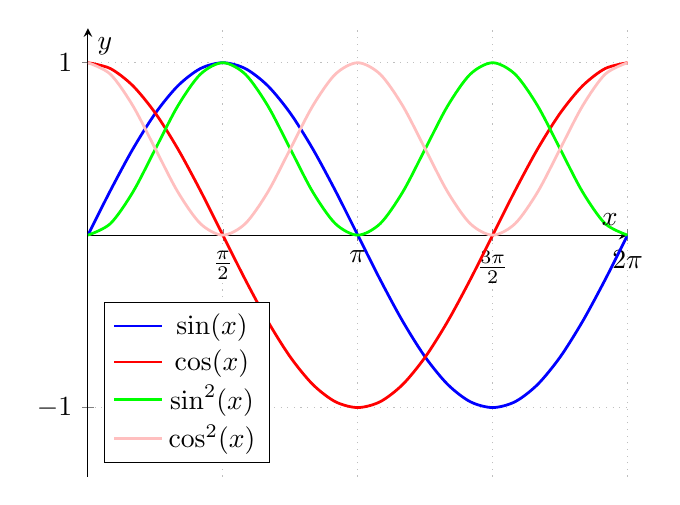
\begin{tikzpicture}
        \begin{axis}[
            domain=0:2*pi,  % Adjusted domain to [0, 2*pi]
            xmin=0, xmax=2*pi,
            ymin=-1.4, ymax=1.2,
            axis lines=middle,
            xlabel={$x$},
            ylabel={$y$},
            xtick={0,1.5708,3.1416,4.7124,6.2832},  % Adjusted xticks for [0, 2*pi]
            xticklabels={$0$,$\frac{\pi}{2}$,$\pi$,$\frac{3\pi}{2}$,$2\pi$},  % Adjusted xtick labels
            ytick={-1,0,1},
            legend pos=south west,
            grid=both,
            grid style={dotted},
        ]

        % Plot sine function
        \addplot[blue,smooth, line width = 1pt] {sin(deg(x))};
        \addlegendentry{$\sin(x)$};

        % Plot cosine function
        \addplot[red,smooth, line width = 1pt] {cos(deg(x))};
        \addlegendentry{$\cos(x)$};

        % Plot sine function
        \addplot[green,smooth, line width = 1pt] {(sin(deg(x)))^2};
        \addlegendentry{$\sin^2(x)$};

        % Plot cosine function
        \addplot[pink,smooth, line width = 1pt] {(cos(deg(x)))^2};
        \addlegendentry{$\cos^2(x)$};

        \end{axis}
    \end{tikzpicture}
    \caption{Sine 和 Cosine 函数在 $[0, 2\pi]$ 的图像}
    \label{fig:sin-and-cos-in-0topi}
\end{figure}

由图\ref{fig:sin-and-cos-in-0topi}
可以归纳出,在区间 $[0,\pi]$ 上三角函数的对称性。
进而可以帮助简化积分的计算。

\subsection{和圆有关的}
\label{definite-integral-about-circle-area}

利用定积分几何意义可知:
\begin{align}
    \int_0^{a}  \sqrt{a^2 - x^2} \mathrm dx &= \dfrac{\pi}{4} a^2 \quad,(a > 0) \label{eq:unit-circle-1-for-integral-evaluation}\\
    \int_0^{a}  \sqrt{2ax - x^2} \mathrm dx &= \dfrac{\pi}{4} a^2 \quad,(a > 0) \label{eq:unit-circle-2-for-integral-evaluation}\\
    \int_0^{2a} \sqrt{2ax - x^2} \mathrm dx &= \dfrac{\pi}{2} a^2 \quad,(a > 0) \label{eq:unit-circle-3-for-integral-evaluation}
\end{align}
其中,
\begin{itemize}
    \item 公式\ref{eq:unit-circle-1-for-integral-evaluation}是一个圆心在$(0, 0)$上的,半径为 $a$ 的$(1/4)$圆的面积;
    \item 公式\ref{eq:unit-circle-2-for-integral-evaluation}是一个圆心在$(a, 0)$上的,半径为 $a$ 的$(1/4)$圆的面积;
    \item 公式\ref{eq:unit-circle-3-for-integral-evaluation}是一个圆心在$(a, 0)$上的,半径为 $a$ 的$(1/2)$圆的面积;
\end{itemize}
% TODO 用 tikz 绘制几个示意图应该效果更好

\subsection{和三角函数奇偶性有关的}

\begin{align}
    \int_0^{\pi} \sin^n x \mathrm{d}x &= 2 \int_0^{\pi/2} \sin^n x \mathrm{d}x \\
    \int_0^{\pi} \cos^n x \mathrm{d}x &= 
    \left\{
        \begin{array}{rl}
            0,                                       &n \mbox{\small \ is odd} \\
            2 \int_{0}^{\pi/2} \cos^n x \mathrm{d}x, &n \mbox{\small \ is even}
        \end{array}
    \right.
\end{align}
这两个公式要结合函数的奇偶性和图像进行深入了解,参见图 
\ref{fig:sin-and-cos-in-0topi}.
两个公式右侧可进一步使用公式\ref{eq:launching-formula}进行求值。
例题参见 \cite[page 108, pdf 119, exmaple 3]{we}.

\subsection{三角函数的线性组合之比的积分}

即形如:
\[
    I = \int \dfrac{a \sin x + b \cos x}{c \sin x + d \cos x}\mathrm{d}x
\]
的,可用下面的待定系数方法简化运算
\begin{equation}
    I = \int 
    \dfrac{
         A(\overbrace{c \cos x - d \sin x}^{\mbox{\small 分母的导数}})
        +B(\overbrace{c \sin x + d \cos x}^{\mbox{\small 分母}})
    }{c \sin x + d \cos x} \mathrm{d}x
\end{equation}
其中$A, B$可以通过令两个分子相等解出。
参见\cite[page 110, pdf 121, example 8]{we}.

\subsection{积分上下限重现换元法}
\label{integral-limits-regenerating-substituting}

这个办法就是通过巧妙地选取换元变量,
是的换元前后的定积分上下限不变,
这样就有
\[
    I = \int_a^b f_1(x) \mathrm{d}x = \int_a^b f_2(t) \mathrm{d}t
\]
其中 $f_2(t)$ 是换元之后的 $f_1(x)$, $x = a + b - t$。
则
\[
    I = \dfrac{1}{2} \int_a^b 
    \underbrace{f_1(x) + f_2(x)}_{{\mbox{\small 这里可以消去一些麻烦}}}
    \mathrm{d}x
\]
只在原函数很难找到的使用,不是万金油。
另外对于多元函数积分利用该方法之前要先用被积函数变量对称性来对积分进行处理,
请参考小节\ref{multivariable-integral-properity-of-variable-symtric}.

参见\cite[page 110, pdf 121, example 8]{we}.

\begin{example}
    \[
        I = \int_0^{\pi} \dfrac{x |\sin x \cos x|}{1+\cos^2 x} \mathrm{d}X
    \]
    \cite[question 64]{w660}
\end{example}

另外还有一种类似的pattern也适合本方法。
令 $x = -x$
\[
    I = \int_{-a}^{a} f(x) \mathrm{d}x = \int_{-a}^{a} f(-t) \mathrm{d}t
\]
得到
\[
    2I = \int_{-a}^{a} \left[f(x) + f(-x)\right] \mathrm{d}x
\]

\subsection{关于 x 的边上限积分等式,求f(x)的定积分}
\begin{enumerate}
    \item 等式两边求导得到关系式
        \begin{itemize}
            \item 有参数在被积函数中存在形式形如$xf(x - t)$的,
                  首先进行换元,
                  使得被积函数转换为形如$(x - u)f(u)$的形式,
            \item 然后再进行拆项求积分
        \end{itemize}
    \item 带点进去关系式
\end{enumerate}

\begin{example}
    \[
        I = \int _0^{\pi/2} \dfrac{\sin x}{\sin x + \cos x} \mathrm{d}x 
    \]
    \cite[page 111, pdf 122, example 10]{we}.

    令 $x = \frac{\pi}{2} + 0 - t$, $\mathrm{d}t = -t$
    \footnote{这里的积分上下限应当倒转,但是有一个 $-1$ 直接又给倒回来了。}

    \begin{align*}
        &\int_0^{\pi/2} \dfrac{\sin x}{\sin x + \cos x} \mathrm{d}x 
        = \int_0^{\pi/2} \dfrac{\cos t}{\sin t + \cos t} \mathrm{d}t \\ 
        = &\dfrac{1}{2} 
        \left(
            \int_0^{\frac{\pi}{2}} 
            \dfrac{\sin x}{\sin x + \cos x} \mathrm{d}x 
            + \int_0^{\frac{\pi}{2}} 
            \dfrac{\cos x}{\sin x + \cos x} \mathrm{d}x
        \right) \\
        = &\dfrac{1}{2} \int_0^{\pi/2} \mathrm{d}x = \dfrac{\pi}{4}
    \end{align*}
\end{example}

\subsection{累次积分计算}

\begin{definition}[累次积分交换次序]
    \begin{align*}
         &\int_a^b \mathrm{d}x \int_{\phi_1(y)}^{\phi_2(y)} 
         f(x, y) \mathrm{d}y \\[1em]
        =&\int_a^b
        \left[
            \int_{\phi_1(y)}^{\phi_2(y)} f(x, y) \mathrm{d}y
        \right] \mathrm{d}x
    \end{align*}
\end{definition}

\begin{example}
    计算二次积分$\int_0^1 \mathrm{d}x \int_{x^2}^{x} xy^2 \mathrm{d}y$
    \begin{align*} 
        &\int_{0}^{1} \text{d}x \int_{x^2}^{x} xy^2 \text{d}y  \\
        = &\int_{0}^{1} 
        \left[ 
            \int_{x^2}^{x} xy^2 \text{d}y 
        \right] 
        \text{d}x 
        = \int_{0}^{1} 
        \left[ 
            \frac{xy^3}{3} 
        \right]_{x^2}^{x} \text{d}x \\ 
        =& \frac{1}{3} \int_{0}^{1} (x^4 - x^7) \text{d}x 
        = \frac{1}{3} 
        \left[ 
            \frac{x^5}{5} - \frac{x^8}{8} 
        \right]_{0}^{1} \\ 
        =& \frac{1}{3} \cdot \frac{3}{40} = \frac{1}{40}.
    \end{align*}

    \url{https://www.zhihu.com/question/517593800}
\end{example}

\subsection{例题}

\begin{example}\label{example:w660t60}
    \[
        I = \int_0^1 \left(\sqrt{\underbrace{2x-x^2}_{-(x-1)^2\mbox{\small 的一部分}}} 
        - \underbrace{\sqrt{(1-x^2)^3}}_{\mbox{\small 出现}\sqrt{a^2-x^2}\mbox{\small 形}}\right) \mathrm{d}x
    \]

    \cite[page 24, question 60]{w660}

    上面第二个大括号提示请参见表 \ref{tab:useful-sec-type-substitutions}.
    按照表中提示,令 $x = \sin t$,那么
    \begin{align*}
        \int_0^1 \left(
            \sqrt{(1-x^2)^3}
        \right) \mathrm{d}x
        &=
        \int_0^1 
            \cos^4 x
        \mathrm{d}x\\
        &=
        \frac{3}{4} \times \frac{1}{2} \times \frac{\pi}{2} = \frac{3}{16} \pi
    \end{align*}
    之后可运用点火公式 \ref{eq:launching-formula} 计算高次幂三角函数。

    式子中的前面一部分的化简目标为单位元面积,
    参见小节 \ref{definite-integral-about-circle-area}。
    则令 \[t = (x-1)\] 则 $2x-x^2 = 1-t^2$
    \[
        \int_0^1 \sqrt{2x-x^2} \mathrm{d}x
        = 
        \int_{-1}^0 \sqrt{1-t^2} \mathrm{d}t = \frac{\pi}{4}
    \]
    
    那么 \[I = \dfrac{\pi}{4} - \dfrac{3\pi}{16} = \dfrac{\pi}{16}\]
\end{example}

\begin{example}
    \[
        I = \int_0^1 \arcsin x \cdot \arccos x \mathrm{d}x
    \]
    \cite[page 24, question 59]{w660}
    一个方法是代换 $t = \arcsin x$ 之后进行分部积分。

    另外一个方法是直接对$I$进行分部积分。可以得到
    \begin{align*}
        I &= \left. \arccos x \arcsin x \right|^{1}_{0} 
             - \int_0^1 x \mathrm{d} \arcsin x \arccos x \\
          &= - \int_0^1 x 
          \left(
              \dfrac{\arccos x}{\sqrt{1-x^2}} 
              - \dfrac{\arcsin x}{\sqrt{1-x^2}}
          \right)
          \mathrm{d}x \\
          &= - 
          \left(
              \underbrace{
                  \int_0^1
                      \dfrac{\arccos x}{\sqrt{1-x^2}} \cdot x
                  \mathrm{d}x 
              }_{A}
              -
              \underbrace{
                  \int_0^1
                      \dfrac{\arcsin x}{\sqrt{1-x^2}} \cdot x
                  \mathrm{d}x 
              }_{B}
          \right) \\[1em]
        A &= - \int_0^1 \arccos x \, \mathrm{d} \sqrt{1-x^2} \\
          &= \left.- \arccos x \sqrt{1-x^2}\right]_0^1 + \int_0^1 \sqrt{1-x^2} \cdot 
              \dfrac{-\mathrm{d}x}{\sqrt{1-x^2}} \\
          &= - \dfrac{\pi}{2} + 1 
    \end{align*}
    同理可得 $B = 1, I = -\dfrac{\pi}{2} + 2$.
\end{example}

\begin{example}
    \[
        I = \int \dfrac{1}{1+\cos x} \mathrm{d}x 
          = \dfrac{1}{2} \int \sec^2 \dfrac{t}{2} \mathrm{d}t
    \]
\end{example}

\begin{example}
    \[
        I = \int_0^{\pi/2} \dfrac{1}{(\sin x + \cos x)^2} \mathrm{d}x
    \]

    Solution1:
    \begin{align*}
        I &= \int_0^{\pi/2} \dfrac{1}{1 + \sin 2x} \mathrm{d}x\\
          &= \dfrac{1}{2} \int_{0}^{\pi} \dfrac{1}{1+\sin x} \mathrm{d}x\\
          &= \dfrac{1}{2} \int_{\pi/2}^{\pi + \pi/2} \dfrac{1}{1+\cos x} \mathrm{d}x \quad (\mbox{\small 诱导公式})\\
          &\mbox{D.N.E}
    \end{align*}
    该解法无法求得定积分,因为被积函数在积分区间上有无穷间断点。如下图所示
    \begin{figure}[H]
        \centering
        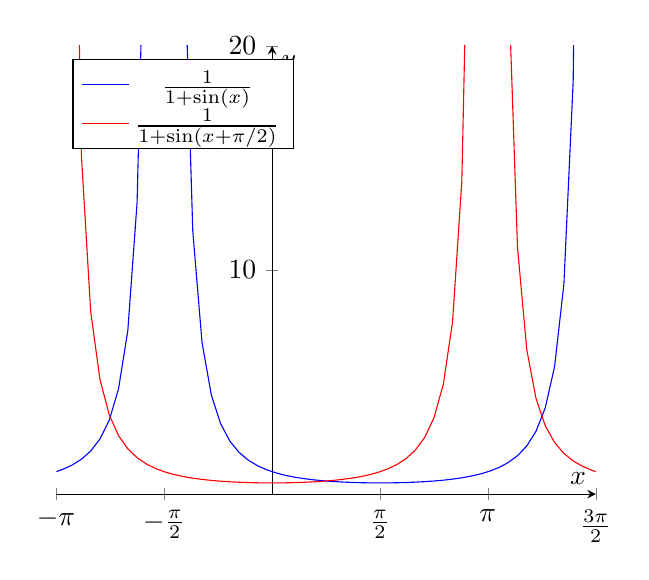
\begin{tikzpicture}
            \begin{axis}[
                axis lines=middle,
                xlabel={$x$},
                ylabel={$y$},
                xmin=-pi,
                xmax=3*pi/2,
                ymin=0,
                ymax=20,
                xtick={-pi,-pi/2,0,pi/2,pi,3*pi/2},
                xticklabels={$-\pi$,$-\frac{\pi}{2}$,$0$,$\frac{\pi}{2}$,$\pi$,$\frac{3\pi}{2}$},
                ytick={0,10,20},
                legend pos= north west,
                domain=-270:270, % Use degrees instead of radians
                restrict y to domain = 0:1000,
                samples=4000,    % Increase the number of samples for smoothness
            ]

            % Function 1
            \addplot[blue] {1/(1 + sin(deg(x)))};
            \addlegendentry{$\frac{1}{1 + \sin(x)}$}

            % Function 2
            \addplot[red] {1/(1 + sin(deg(x) + 90))}; % 90 degrees is equivalent to pi/2 radians
            \addlegendentry{$\frac{1}{1 + \sin(x + \pi/2)}$}

            \end{axis}
        \end{tikzpicture}
    \end{figure}
    所以在凑微分 $\sec^2 x$ 的时候要注意积分区间内是否出现无穷间断点。

    Solution2:
    \begin{align*}
        I &= \int_0^{\pi /2} \dfrac{1}{\left[\sqrt{2} \sin \left(x+\dfrac{\pi}{4}\right)\right]^2} \mathrm{d}x \\
          &= \dfrac{1}{2} \int_0^{\pi/2} \sec^2 \left(x-\dfrac{\pi}{4}\right)\mathrm{d} x-\dfrac{\pi}{4}\\
          &= \left. \dfrac{1}{2} \tan \left(x - \dfrac{\pi}{4}\right) \right]^{\pi/2}_{0}
    \end{align*}
    解法2应用了辅助角公式,但是在这里,并没有体现辅助角。
\end{example}

\section{变上限积分积分及其应用}

考点:
\begin{itemize}
    \item 变上限积分的连续性
    \item 变上限积分的可导性
    \item 边上限积分的奇偶性
\end{itemize}

变限积分在计算的时候可以利用 小节\ref{limit-rerepresenting-in-variable-limits-integral}。

\subsection{常用结论和符合直觉的原因}

\subsubsection{连续性和可导性}

\begin{theorem}
    若 $f(x)$ 在 $[a, b]$ 上可积,则 $\int_a^x f(x) \mathrm{d} t$
    在 $[a, b]$ 上连续。
\end{theorem}

\begin{theorem}
    \label{thm:derivative-of-variadict-integral}
    若 $f(x)$ 在 $[a, b]$ 上连续,则 $\int_a^x f(x) \mathrm{d} t$
    在 $[a, b]$ 上可导,且
    \[
        \left(\int_a^x f(t) \mathrm{d}t\right)' = f(x)
    \]
\end{theorem}

\begin{corollary}
    \label{co:derivative-of-variadict-integral-corollary}
    若 $f(x)$ 在 $[a, b]$ 上连续;$g, h$ 在 $(a, b)$ 上可导, 
    则 $\int_{h(x)}^{g(x)} f(x) \mathrm{d} t$
    在 $[a, b]$ 上可导,且
    \[
        \left(\int_{h(x)}^{g(x)} f(t) \mathrm{d}t\right)' = 
        f(g(x))g'(x) - f(h(x))h'(x)
    \]
\end{corollary}

\begin{example}
    \[
        \dfrac{\mathrm d}{\mathrm dx} \int_{2x}^{\ln x} \ln(1+t) \mathrm dt
    \]
    \cite[question 192]{w660}.
    \begin{align*}
        &\dfrac{\mathrm d}{\mathrm dx} \int_{2x}^{\ln x} \ln(1+t) \mathrm dt \\
        =&\ln(1+\ln x)(\ln x)' - \ln(1+2x)(2x)'\\
        =&\frac{1}{x} \ln (1+\ln x) - 2\ln (1+2x)
    \end{align*}
\end{example}

\begin{table}
    \centering
    \begin{tabular}{cc}
        \toprule
        $f(x)$ & $F(x) = \int_a^x f(x) \mathrm{d}x$ \\
        \midrule
        连续             & 可导,$F'(x) = f(x)$ \\
        有限个可去间断点 & 可导,$F'(x) = \lim_{x \to x_0} f(x)$\\
        有限个跳跃间断点 & 连续但不一定可导,\\
        {}&$F_{-}'(x) = f({x_0}_{-}), F_{+}'(x) = f({x_0}_{+})$ \\
        \bottomrule
    \end{tabular}
    \caption{在\textbf{某点处}变上限积分的某些常用性质}
    \label{tab:useful-properoties-of-variable-limits-integral}
\end{table}

表 \ref{tab:useful-properoties-of-variable-limits-integral} 中
有限个可去间断点对函数和座标轴的面积没有影响。因此$F(x)$是可导的,
但是其值确实该点处$f(x)$的极限值。
跳跃间断点两处函数求极限不一定相等,因此不能推出可导。

\subsubsection{奇偶性}

若 $f(x)$ 连续,则
\begin{itemize}
    \item 若$f(x)$为奇函数,则$\int_a^x f(x) \mathrm{d}x$ 为偶函数。
    \item 若$f(x)$为偶函数,则$\int_0^x f(x) \mathrm{d}x$ 为奇函数。
\end{itemize}
请注意,上面第二条中的积分下限为$0$,而不是任意常数 $a$.

\subsubsection{例子}

\begin{example}
    设 $g(x) = \int_a^x f(u) \mathrm{d} u$ 其中
    \[
        f(x) = \left\{
            \begin{array}{rl}
                \dfrac{1}{2} (x^2+1),\, \mbox{if}\, 0 \leq x \leq 1, \\[1em]
                \dfrac{1}{3} (x-1),  \, \mbox{if}\, 1 \leq x \leq 2.
            \end{array}
        \right.
    \]
    则$g(x)$在$(0, 2)$内

    A.无界\quad B.连续\quad C.连续 \quad D.不连续

    这个题目首先,一个函数要么是连续的要么是不连续的,
    所以答案肯定是在 C 和 D 中。
    当 $x \to 1$, $\frac{1}{2} (x^2 + 1) \to 1$ 
    另外 $\frac{1}{3} (x - 1) \to 0$
    在区间$(0,2)$上存在一个跳跃间断点,则$f(x)$肯定是可积的.
    则$f(x)$的变上限积分肯定是连续函数。

    本题目考察了变上限积分的连续性,传统做法将分段函数的积分算出来,
    再考察连续性,速度就会慢很多。
\end{example}

\begin{example}
    \label{example-limits-and-varidic-limits-integral-2}
    设函数 $f(x)$ \textbf{连续},且$f(0) \neq 0$,求
    \[
        L = \lim_{x \to 0} \dfrac{\int_0^x (x - t) f(t) \mathrm dt }{x \int_0^x f(x - t) \mathrm dt}
    \]
    \cite[page 114, pdf 125]{we}
    \begin{align}
        &\int_0^x f(x - t) \mathrm dt = \int_0^x f(u) \mathrm du \quad (\mbox{令} x - t = u)\notag \\
        L =& \lim_{x \to 0} \dfrac{x \int_0^x f(t) \mathrm dt - \int_0^x tf(t) \mathrm dt}{x \int_0^x f(t) \mathrm dt}\notag \\
          =& \lim_{x \to 0} \dfrac{\int_0^x f(t) \mathrm dt + xf(x) - x(f)}{\int_0^x f(t) \mathrm dt + xf(x)} \quad (\mbox{\small L'Hospital}) \notag\\
          =& \lim_{x \to 0} \dfrac{\int_0^x f(t) \mathrm dt}{\int_0^x f(t) \mathrm dt + xf(x)} \quad \label{eq:part-no-L-Hospital-1}\\
          =& \lim_{x \to 0} \dfrac{xf(c)}{xf(c) + xf(x)}\quad(c \in (0, x)) \label{eq:part-mid-value-theorm-1}\\
          =& \dfrac{f(0)}{f(0) + f(0)} = \dfrac{1}{2} \notag
    \end{align}
    
    另解
    \[
        L =\lim_{x \to 0} \dfrac{x \int_0^x f(t) \mathrm dt - \int_0^x tf(t) \mathrm dt}{x \int_0^x f(t) \mathrm dt}
    \]
    由 $f(0) \neq 0$ 得,当$x\to 0$时\footnote{参见小节\ref{limit-questions-involved-definite-integral}和\ref{limit-rerepresenting-in-variable-limits-integral}}:
    \begin{align*}
        \int_0^x f(t) \mathrm dt  &\sim \int_0^x  f(0) \mathrm dt = f(0) x \\
        \int_0^x tf(t) \mathrm dt &\sim \int_0^x tf(0) \mathrm dt = \dfrac{f(0)}{2} x^2
    \end{align*}
    则
    \begin{equation*}
        L = 1 - \lim_{x\to 0} \dfrac{\int_0^x tf(t) \mathrm dt}{x \int_0^x f(t) \mathrm dt} 
          = 1 - \lim_{x\to 0} \dfrac{\frac{f(0)}{2} x^2}{f(0) x^2} = \dfrac{1}{2}
    \end{equation*}

    另外还有一种解法利用了广义积分中值定理\footnote{参见 Theorem \ref{general-mean-value-theorm-of-integral}}
    \begin{align}
        L &= \lim_{x \to 0} \dfrac{f(\xi)\int_0^x (x - t) \mathrm dt}{x^2 f(x - c)} \quad (\xi, c \in [0, x])\label{eq:example-part-general-mid-val-theorm-of-integral-1} \\
          &= \lim_{x \to 0} \dfrac{\int_0^x (x - t) \mathrm dt}{x^2} \label{eq:example-part-general-mid-val-theorm-of-integral-2} \\
          &= \lim_{x \to 0} \dfrac{\frac{1}{2} x^2}{x^2} = \dfrac{1}{2} \notag
    \end{align}
\end{example}
上例中步骤(\ref{eq:part-no-L-Hospital-1}) 不可使用L'Hospital法则,
原因是提干中只说明$f(x)$连续,是可导的充分非必要条件。
若此处应用 L'Hospital 法则将会出现 $f'(x)$.
为了继续消除积分符号,可以利用积分中值定理\footnote{参见\ref{general-mean-value-theorm-of-integral}}
,如步骤(\ref{eq:part-mid-value-theorm-1})和(\ref{eq:example-part-general-mid-val-theorm-of-integral-1}).

积分中值定理的缘故,有 
\[
    \lim_{x \to 0} 
    \dfrac{
        \overbrace{f(\xi)}^{\mathclap{=f(0) \neq 0}}
    } {
        \underbrace{f(x - c)}_{\mathclap{=f(0)\neq 0}}
    } = 1
\]
因此步骤(\ref{eq:example-part-general-mid-val-theorm-of-integral-2})成立。

本例第一个解的前几行是将积分上下限同被积函数变量分离的技术。
其他有关变限积分被积函数中出现积分上下限的例子,还请参考
例\ref{example-limits-and-varidic-limits-integral-1}.

\section{积分不等式}

本考点出的题目可以是整张卷子中最难的题目,

可能用到的知识点:
\begin{itemize}
    \item 定积分不等式性质
        \begin{itemize}
            \item 三个不等式性质
            \item 积分中值定理
        \end{itemize}
    \item 变量代换
    \item 积分中值定理
    \item 变上限积分
    \item Cauchy 积分不等式
\end{itemize}

其中,
将定积分不等式用变上限积分表达,
就将定积分(值)不等式转换为边上限积分(函数)不等式。

选择题方法:
\begin{itemize}
    \item 直接比较被积函数大小 
    \item 带入特殊点
    \item 使得被积函数 $\to 0$ 然后进行等价代换后,重复执行上面的方法。
\end{itemize}

\begin{theorem}[Cauchy 积分不等式]\label{Cauchy-integral-inequlity}
    \[
        \left(\int_a^b f(x)g(x) \mathrm{d}x\right)^2 
        \leq 
        \int_a^b f^2(x) \mathrm{d}x\, \int_a^b g^2(x) \mathrm{d}x
    \]
    注意观察,柯西积分不等式将平方从积分上移动到了积分内部。
\end{theorem}

\begin{example}
    \begin{align*}
        I_1 &= \int_0^1 \dfrac{x}{2(1+\cos x)} \mathrm{d}x     &= \int_0^1 f(x) \mathrm{d}x \\
        I_2 &= \int_0^1 \dfrac{\ln(1+x)}{1+\cos x} \mathrm{d}x &= \int_0^1 g(x) \mathrm{d}x \\
        I_3 &= \int_0^1 \dfrac{2}{1+\sin x} \mathrm{d}x        &= \int_0^1 h(x) \mathrm{d}x \\
    \end{align*}
    比较上面三个式子大小。

    本题目三个积分的上下限均相等,则被积函数的大小关系即可认为是积分的大小关系。

    三种解法:
    \begin{itemize}
        \item 传统办法:基本不等式比较函数大小
        \item 带入特殊点
        \item 使得 $x\to 0$ 比较被积函数等价无穷小
            \[
                x \to 0^+, f(x) \to \dfrac{x}{4}, g(x) \to \dfrac{x}{2}, h(x) \to 2x.
            \]
    \end{itemize}
\end{example}

\begin{example}
    \begin{align*}
        M &= \int_{-\frac{\pi}{2}}^{\frac{\pi}{2}} \frac{(1+x)^2}{1+x^2} \mathrm dx \\
        N &= \int_{-\frac{\pi}{2}}^{\frac{\pi}{2}} \frac{1+x}{e^x} \mathrm dx \\
        K &= \int_{-\frac{\pi}{2}}^{\frac{\pi}{2}} (1+\sqrt{\cos x})\mathrm dx 
    \end{align*}
    请比较上述三个积分的大小.

    \cite[question 184]{w660}.

    \begin{align*}
        M &= \int_{-\frac{\pi}{2}}^{\frac{\pi}{2}} \frac{(1+x)^2}{1+x^2} \mathrm dx 
           = \int_{-\frac{\pi}{2}}^{\frac{\pi}{2}} \frac{1+x^2+2x}{1+x^2} \mathrm dx \\
          &= \int_{-\frac{\pi}{2}}^{\frac{\pi}{2}} 1 \mathrm dx 
          + \int_{-\frac{\pi}{2}}^{\frac{\pi}{2}} \underbrace{\frac{2x}{1+x^2}}_{\mathclap{\mbox{\small 函数关于原点对称}}} \mathrm dx = \pi
    \end{align*}
    因为\footnote{基本不等式参见小节 \ref{inequlity}} $e^x > 1+x$, 
    \[
        N = \int_{-\frac{\pi}{2}}^{\frac{\pi}{2}} \frac{1+x}{e^x} \mathrm dx < 
        \int_{-\frac{\pi}{2}}^{\frac{\pi}{2}} 1 \mathrm dx 
        = \pi
    \]
    又因为 
    \begin{gather*}
        1+\sqrt{\cos x} \geq 1\\ x \in \left(-\frac{\pi}{2}, \frac{\pi}{2}\right)\\
        K = \int_{-\frac{\pi}{2}}^{\frac{\pi}{2}} (1+\sqrt{\cos x})\mathrm dx > 
        \int_{-\frac{\pi}{2}}^{\frac{\pi}{2}} 1 \mathrm dx 
        = \pi
    \end{gather*}
    综上\footnote{题目用一个 $\pi$ 联系了起来} $K>M>N$.
\end{example}

大题考法\footnote{列举出的方法是在题目中都要使用的方法}:
\begin{itemize}
    \item 函数单调性方法
        \begin{enumerate}
            \item 变形为变上限积分
            \item 判断函数(变上限积分)单调性,通过积分中值定理将函数的大小比较转换为函数上两个点的大小比较。
        \end{enumerate}
    \item 转换不等号两边积分上下限相同,比较被积函数。
    \item 直接利用积分不等式性质。
\end{itemize}

\begin{example}
    Suppose $f(x)$ is continuous on $[0,1]$, 单调减函数,求证:
    \[
        \int_0^a f(x) \mathrm{d}x \leq a \int_0^1 f(x) \mathrm{d}x, \quad a \in (0, 1)
    \]
    \cite[page 119, pdf 130, example 2]{we}

    Solution1:
    \begin{proof}
        将不等号右边写为
        \[
            a\int_0^a f(x) \mathrm{d}x + a\int_a^1 f(x) \mathrm{d}x
        \]
        然后移项,则原式子变为:
        \[
            (1-a) \int_0^a f(x) \mathrm{d}x \leq a \int_a^1 f(x) \mathrm{d}x,
        \]
        由积分中值定理\footnote{\ref{general-mean-value-theorm-of-integral}}可知
        \begin{align}
            (1-a) \int_0^a f(x) \mathrm{d}x = a(1-a)f(\xi_1), \quad \xi_1 \in (0, a)\\
            a \int_a^1 f(x) \mathrm{d}x = a(1-a)f(\xi_2), \quad \xi_2 \in (a, 1)
        \end{align}
        又因为 $f(x)$ 单调减,则$f(\xi_1) > f(\xi_2)$,从而
        \[
            (1-a) \int_0^a f(x) \mathrm{d}x \leq a \int_a^1 f(x) \mathrm{d}x,
        \]
    \end{proof}

    Solution2:
    \begin{proof}
        let $F(a) = \int_0^a f(x) \mathrm{d}x - a\int_0^1 f(x) \mathrm{d}x, (0 \leq a \leq 1)$,则
        \[
            F'(a) = f(a) -  \int_0^1 f(x)\mathrm{d}x = f(a) - f(\xi), \xi \in (0,1)
        \]
        由于 $f(x)$ 单调减,则当 $0<a<c$ 时,$F'(a) > 0$.
        $F(a)$ 单调增;
        当 $a<c<1$ 时,$F'(a) < 0$.
        $F(a)$ 单调减.
        则$F(a)$在区间$[0,1]$上的最小值必在区间的端点取到,
        又因为 $F(0) = F(1) =0$ 则
        \[
            F(a) \leq 0, \quad a \in (0, 1)
        \]
    \end{proof}
    该方法即为将桉树转换为变上限积分函数后应用函数单调性解题的。
\end{example}

题目给单调性条件后才能用这种办法。
在书写过程的时候要注意说明自变量的单调性,
然后是函数的单调性,这样才能说明整个式子的性质。
其他例子请参见 \cite[page 119, pdf 130]{we}.

\begin{example}
    求证
    \begin{gather}
        \label{exeq:prof1-quiz} \int_0^{2\pi} \dfrac{\sin x}{x} \mathrm dx > 0 \\
        \label{exeq:prof2-quiz} \int_0^{2\pi} \cos x \ln ( 2+ \cos x) \mathrm dx > 0 \\
        \label{exeq:prof3-quiz} \int_0^{\frac{\pi}{2}} \dfrac{\sin x}{x} \mathrm dx > 1
    \end{gather}

    \cite[question 183]{w660}.

    \begin{proof}[Proof of \ref{exeq:prof1-quiz}]
        \begin{align*}
            \int_0^{2\pi} \dfrac{\sin x}{x} \mathrm dx
            &= \int_0^{\pi} \dfrac{\sin x}{x} \mathrm dx 
            + \int_{\pi}^{2\pi} \dfrac{\sin x}{x} \mathrm dx \\
            &= \int_0^{\pi} \dfrac{\sin x}{x} \mathrm dx 
            + \int_{0}^{\pi} \dfrac{\sin (x + \pi)}{x + \pi} \mathrm dx \\
            &= \int_0^{\pi} \dfrac{\sin x}{x} \mathrm dx 
            - \int_{0}^{\pi} \dfrac{\sin x }{x + \pi} \mathrm dx \\
            &= \int_0^{\pi} \dfrac{\pi \sin x}{x(x + \pi)} \mathrm dx  > 0
        \end{align*}
    \end{proof}

    \begin{proof}[Proof of \ref{exeq:prof2-quiz}]
        由于被积函数是以 $2\pi$ 为周期的偶函数,所以
        \begin{align*}
            &\int_0^{2\pi} \cos x \ln ( 2+ \cos x ) \mathrm dx \\
            =&\int_{-\pi}^{\pi} \cos x \ln ( 2+ \cos x ) \mathrm dx \\
            =&2\int_{0}^{\pi} \cos x \ln ( 2+ \cos x ) \mathrm dx \\
            =&2\left[
                \splitfrac{
                    \int_0^{\pi/2} \cos x \ln ( 2+ \cos x ) \mathrm dx
                }{
                    + 
                    \underbrace{\int_{\pi/2}^{\pi} \cos x \ln ( 2+ \cos x ) \mathrm dx}_{I_1}
                }
            \right]
        \end{align*}
        对 $I_1$ 做积分变量变换 $x = \pi - t$ 则
        \[
            I_1 = \int_0^{\frac{\pi}{2}} \cos t \ln ( 2+ \cos t ) \mathrm dt 
        \]
        所以
        \begin{align*}
            &\int_0^{2\pi } \cos x \ln (2 + \cos x) \mathrm dx \\
            =&2 \int_0^{\frac{\pi}{2}} \cos x \ln \dfrac{2+ \cos x}{2- \cos x} \mathrm dx > 0
        \end{align*}
    \end{proof}

    \begin{proof}[Proof of \ref{exeq:prof3-quiz}]
        有
        \[
            RHS = 1 = \int_0^{\frac{\pi}{2}} \dfrac{2}{\pi} \mathrm dx
        \]
        令
        \[
            \varphi(x) = \frac{\sin x}{x} -\frac{2}{\pi}, \quad x \in \left(0, \frac{\pi}{2}\right)
        \]
        有
        \begin{align*}
            \varphi\left(\frac{\pi}{2}\right) &= 0, \\
            \varphi'(x) &= \dfrac{x \cos x - \sin x}{x^2}\\
                        &= \dfrac{\cos x \overbrace{(x - \tan x)}^{\mathclap{<0 \mbox{\small, See Figure \ref{fig:tanx-x}}}}}{x^2} < 0
        \end{align*}
        所以当 $x \in \left(0, \frac{\pi}{2}\right)$ 时 $\varphi(x)>0$
        即
        \begin{align*}
            &\dfrac{\sin x}{x} > \dfrac{2}{\pi}, \quad x \in \left(0, \frac{\pi}{2}\right) \\
            \Rightarrow &\int_0^{\frac{\pi}{2}} \dfrac{\sin x}{x} \mathrm dx > \int_0^{\frac{\pi}{2}} \dfrac{2}{\pi} \mathrm dx = 1
        \end{align*}
    \end{proof}
\end{example}

\begin{figure}
    \centering
    \includegraphics[width=0.5\textwidth]{figure/tanx-x.pdf}
    \caption{The figure of $\tan x$ and $x$, to illustrate $\tan x > x, x \in (0, \pi/2)$.}
    \label{fig:tanx-x}
\end{figure}

\section{定积分的应用}\label{app-finite-integral}

利用定积分定义求极限请参见
Section \ref{use-squeeze-or-definition-of-integral}.

其他定积分的应用请参考
\cite[page 435]{stewart}等参考书.

\begin{corollary}[旋转体积]
    旋转体体积是对其切面(washer)的面积进行积分得来的。
    而切面的面积可以表示为
    \[
        A(y) = \pi \left[(\mbox{\small outer radius})^2-(\mbox{\small inner radius})^2\right]
    \]
    整个旋转体体积就可以表示为
    \[
        V(y) = \int_a^b A(y) \mathrm dy
    \]
    \cite[page 453]{stewart}.
\end{corollary}

可参考题目 \cite[question 206]{w660}.

\begin{theorem}[The Arc Length Formula]
    If $f'$ is continuous on $[a, b]$, then the length of the curve
    $y = f(x), x \in [a, b]$
    \[
        L = \int_a^b \sqrt{1 + [f'(x)]^2} \mathrm dx
    \]

    \cite[page 561]{stewart}.
\end{theorem}

\begin{theorem}
    \label{thm:length-arc-parametric}
    If a curve $C$ is described by the \uline{parametric equations}
    $x = f(t), y = g(t), t \in [\alpha, \beta]$, where $f'$
    and $g'$ are continuous on $[\alpha, \beta]$ and $C$ is 
    traversed \emph{exactly once} as $t$ increases from $\alpha$ to $\beta$, 
    then the length of $C$ is
    \[
        L = \int_{\alpha}^{\beta} 
        \underbrace{\sqrt{\left(\frac{\mathrm dx}{\mathrm dt}\right)^2 + \left(\frac{\mathrm dy}{\mathrm dt}\right)^2}
        \mathrm dt}_{\mbox{\small 弧微分}}
    \]
\end{theorem}

\begin{corollary}
    According to the Theorem \ref{thm:length-arc-parametric}:
    Assuming $f'$ is continuous, the length of the curve with \uline{polor equation}
    $r = f(\theta), \theta \in [a, b]$ is
    \[
        L = \int_a^b 
        \sqrt{r^2 + \left(\frac{\mathrm dr}{\mathrm d\theta}\right)^2} 
        \mathrm d\theta
    \]
\end{corollary}

摆线的应用看起来也是比较喜欢考察的,
摆线的类型请参见 \cite{stewartpre} 相关章节。

\begin{corollary}[摆线质心]
    摆线质心$(\overline x, \overline y)$就是摆线上所有点的平均位置:
    \begin{align*}
        \overline x &= \dfrac{
            \int_a^b x(t) \overbrace{\sqrt{x'^2(t) + y'^2(t)} \mathrm dt}^{\mbox{\small 弧微分}}
        }{
            \int_a^b \sqrt{x'^2(t) + y'2(t)} \mathrm dt 
        } \\
        \overline y &= \dfrac{
            \int_a^b y(t) \sqrt{x'^2(t) + y'^2(t)} \mathrm dt 
        }{
            \underbrace{\int_a^b \sqrt{x'^2(t) + y'^2(t)} \mathrm dt }_{\mbox{\small 弧长}L}
        } 
    \end{align*}
    其中 $t \in [a, b]$
\end{corollary}

\begin{example}
    \label{ex:centriod-of-curve}
    摆线的一支 
    \begin{align*}
        x &= a(t - \sin t) \\
        y &= a(1 - \cos t) 
    \end{align*}
    $(t \in [0, 2\pi])$的质心是
    
    \cite[question 208]{w660}.

    先求弧微分
    \begin{align*}
        \mathrm ds &= \sqrt{x'^2(t) + y'2(t)} \mathrm dt \\
                   &= \sqrt{(a - a\cos t)^2 + (-a \sin t)^2} \mathrm dt \\
                   &= \sqrt{a^2(1-\cos t)^2 + (a \sin t)^2} \mathrm dt \\
                   &= a\sqrt{(1 - \cos t)^2 + a^2 \sin^2 t} \mathrm dt \\
                   &= a\sqrt{2 - 2 \cos t} \mathrm dt = a\sqrt{2(1 - \cos t)} \mathrm dt \\
                   &= a\sqrt{2(2 \sin^2 \frac{t}{2})} \mathrm dt \\
                ds &= 2a \sin \frac{t}{2} \mathrm dt \quad (t \in [0, 2\pi])
    \end{align*}

    再求弧长
    \begin{align*}
        L&=\int_0^{2 \pi} \sqrt{x'^2(t) + y'2(t)} \mathrm dt \\
         &=\int_0^{2 \pi} 2a \sin \frac{t}{2} \mathrm dt = 4a \left[-\cos \frac{t}{2}\right]^{2\pi}_0 = 8a
    \end{align*}

    \begin{align*}
        \overline y &= \dfrac{
                           \int_a^b y(t) \sqrt{x'^2(t) + y'^2(t)} \mathrm dt 
                       }{
                           \int_a^b \sqrt{x'^2(t) + y'^2(t)} \mathrm dt
                       } \\
                    &= \frac{\overbrace{\int_0^{2 \pi} a(1-\cos t) \overbrace{2a \sin \frac{t}{2} \mathrm dt}^{\mathrm ds}}^{A}}{8a} \\
                  A &= \int_0^{2 \pi} a(2 \sin^2 \frac{t}{2}) 2a \sin \frac{t}{2} \mathrm dt \quad (\mbox{\small Corollary \ref{co:trig-order-raising-equations}})\\
                    &= 4a^2 \int_0^{2\pi} \sin^3 \frac{t}{2} \mathrm dt = 8a^2 \int_0^{\pi} \sin^3 t \mathrm dt \\
                    &= 16a^2 \int_0^{\frac{\pi}{2}} \sin^3 t \mathrm dt \quad (\mbox{\small Launching Formula \ref{eq:launching-formula}})\\
                    &= 16a^2 \cdot \frac{2}{3} = \frac{32}{3}a^2\\
        \overline y &= \frac{A}{8a} = \frac{\frac{32}{3}a^2}{8a} = \frac{4}{3}a
    \end{align*}

    另外这支摆线关于直线 $x = \pi a$ 对称
    \footnote{如图 \ref{fig:figure-of-w660-question-208} 所示。当 $a = 1$ 时,图中加粗线表示 $x = \pi a$} ,
    根据对称性可知 $\overline x = \pi a$
    或者计算 
    \begin{align*}
         &\int_0^{2\pi} x(t) \sqrt{x'^2(t) + y'^2(t)} \mathrm dt \\
        =&\int_0^{2\pi} a(t - \sin t) 2a \sin \frac{t}{2} \mathrm dt \\
        =&-4a^2 \int_0^{2\pi} t \mathrm d \cos \frac{t}{2} - 4a^2 \int_{0}^{2\pi} \sin^2 \frac{t}{2} \cos \frac{t}{2} \mathrm dt \\
        =&-4a^2 t \left.\cos \frac{t}{2}\right]^{2\pi}_0 + 4a^2 \int_0^{2\pi} \cos \frac{t}{2} \mathrm dt \\
         &{\,} -8a^2 \int_0^{2\pi} \sin^2 \frac{t}{2} \mathrm d \sin \frac{t}{2} \\
        =&8a^2 \pi
    \end{align*}

    带入公式得
    \begin{align*}
        \overline x &= \dfrac{
                           \int_0^{2\pi} x(t) \sqrt{x'^2(t) + y'^2(t)} \mathrm dt 
                       }{
                           \int_0^{2\pi} \sqrt{x'^2(t) + y'^2(t)} \mathrm dt
                       } \\
                    &= \frac{8a^2 \pi}{8a} = \pi a.
    \end{align*}
    
    综上,$(\overline x, \overline y) = (\pi a, \frac{4}{3}a)$.
\end{example}

\begin{figure}
    \centering
    \includegraphics[width=0.5\textwidth]{figure/figure-of-w660-question-208.pdf}
    \caption{The figure of $x = (t - \sin t) y = (1 - \cos t)$.}
    \label{fig:figure-of-w660-question-208}
\end{figure}

\section{无界函数反常积分}

\begin{definition}
    若函数 $f(x)$ 在点 $a$ 的任一邻域内都无界,
    那么点 $a$ 称为函数 $f(x)$ 的瑕点。
\end{definition}

\begin{theorem}[比较判别法]
    \label{comparasion-deterministic-informal-integral}
    设$f(x), g(x)$ 在$(a, b]$ 上连续,且
    $0 \leq f(x) \leq g(x)$,$x = a$ 为 $f(x)$ 和 $g(x)$ 的瑕点,则
    \begin{gather*}
        \int_a^b g(x) \mathrm dx \, \mbox{收敛} \Rightarrow \int_a^b f(x) \mathrm dx \, \mbox{收敛} \\
        \int_a^b g(x) \mathrm dx \, \mbox{发散} \Rightarrow \int_a^b f(x) \mathrm dx \, \mbox{发散} 
    \end{gather*}
\end{theorem}

\begin{theorem}[比较判别法的极限形式]
    \label{comparasion-deterministic-informal-integral-limit-form}
    设 $f(x), g(x)$ 在 $(a, b]$ 上非负连续,且
    \[
        \lim_{x \to a^+} \dfrac{f(x)}{g(x)} = \lambda \quad \mbox{(有限或无穷)}
    \]
    则
    \begin{align*}
        \int_a^b f(x) \mathrm dx \mbox{收敛} 
        \Leftrightarrow 
        \int_a^b g(x) \mathrm dx \mbox{收敛} &, \lambda \neq 0 \\
        \int_a^b g(x) \mathrm dx \mbox{收敛} 
        \Rightarrow 
        \int_a^b f(x) \mathrm dx \mbox{收敛} &, \lambda = 0 \\
        \int_a^b g(x) \mathrm dx \mbox{发散} 
        \Rightarrow 
        \int_a^b f(x) \mathrm dx \mbox{发散} &, \lambda = 0
    \end{align*}
\end{theorem}

\begin{corollary}[P积分]
    \label{P-integral}
    \[
        \int_a^b \dfrac{1}{(x - a)^p} \mathrm dx 
        \begin{dcases*}
            \mbox{收敛} & p < 1, \\
            \mbox{发散} & p \geq 1;
        \end{dcases*}
    \]
    \[
        \int_a^b \dfrac{1}{(b - x)^p} \mathrm dx 
        \begin{dcases*}
            \mbox{收敛} & p < 1, \\
            \mbox{发散} & p \geq 1.
        \end{dcases*}
    \]
\end{corollary}

\begin{example}
    证明以下命题不成立
    \begin{enumerate}
        \item 设 $f(x)$ 在 $(-\infty, +\infty)$ 内连续是奇函数,则 $\int_{-\infty}^{+\infty} f(x) \mathrm dx = 0$.
        \item 设 $f(x)$ 在 $(-\infty, +\infty)$ 内连续,$\lim_{R \to +\infty} \int_{-R}^{R} f(x) \mathrm dx$ 存在,则 $\int_{-\infty}^{+\infty} f(x) \mathrm dx$ 收敛.
        \item 若 $\int_{-\infty}^{0} f(x) \mathrm dx$ 与 $\int_0^{+\infty} f(x) \mathrm dx$ 均发散,则不能确定 $\int_{-\infty}^{+\infty}f(x) \mathrm dx$ 是否收敛.
    \end{enumerate}
    
    \cite[question 204]{w660}.

    \begin{proof}[Proof of Proposition 1]
        \begin{align*}
            &\because   \exists f(x) = \sin x \quad \mbox{s.t.} \quad \int_{-\infty}^{+\infty} f(x) \mathrm dx \mbox{\,divergent}\\
            &\therefore \mbox{Proposition invalid.}
        \end{align*}
    \end{proof}

    \begin{proof}[Proof of Proposition 2]
        \begin{align*}
            &\because   \exists f(x) = \sin x \\
            &{\,}\mbox{s.t.} 
                        \int_{-\infty}^{+\infty} f(x) \mathrm dx 
                        \mbox{\,divergent} \\
            &{\,}\bigwedge 
                        \lim_{R \to +\infty} \int_{-R}^{R} f(x) \mathrm dx = 0 \\
            &\therefore \mbox{Proposition invalid.}
        \end{align*}
    \end{proof}

    在 Proposition 3 给定条件下 $\int_{-\infty}^{+\infty}f(x) \mathrm dx$ 发散.
\end{example}


\cleardoublepage
\chapter{Ordinary Differential Equations}
\section{Definition and Terminology} \label{def-de}
We shall classfy differential equations according to 
\textbf{type, order and linearity}

\begin{itemize}
    \item[Types]
        \begin{itemize}
            \item ODE\footnote{Only the ODE is required by NUGEE.}
            \item PDE
        \end{itemize}
    \item[Order]
        The meaning of \textbf{order} is same as the 
        \textbf{order} of differentiation.
    \item[Linearities]
        The meaning of \textbf{degree} is same as the 
        the \textbf{degree} of polynomial.
\end{itemize}

\subsection{Verification of Solutions}

A solution of a differnential equation that is identically zero
on an interval $I$ is said to be a \textbf{trivial solution}.

You have to check the solution of a differential equation wether
or not fit it's interval of definition (domain).

\subsection{Function v.s. Solution}

You have to check the solution of a differential equation wether
or not fit it's interval of definition (domain).

The domain of $y = 1/x$, considered simply as a \textbf{function}, 
is the set of all real numbers $x$ except $0$. 

Now $y = 1/x$ is also a \textbf{solution} 
of the linear first-order differential equation
$xy' + y = 0$. (Verify.) But when we say that $y = 1/x$ 
is a \textbf{solution of this DE}, we
mean that it is a function defined 
\emph{on an interval I} on which it is differentiable and
\emph{satisfies} the equation\cite{fcde}.

\section{First-Order Differential Equations}

The \textbf{critical point} of a autonomous differential equation
is a constant number which satisfy $f(c) = 0$.
Meanwhile, $y(x) = c$ is also a constant solution of the equation.

A critical point is also called \textbf{equilibrium point} or
\textbf{stationary point}.

A constant solution $y(x) = c$ is called an 
\textbf{equilibrium solution}\cite{fcde}.

\subsection{Conclusions of Non-constant Solution of A Autonomous}

\begin{definition}
    [Autonomous differential equation] is a First-Order Differential Equations which like
    \[
        \dfrac{\mathrm{d}y}{\mathrm{d}t} = f(y)
    \]

    Many differential equations encountered in applications or equations that are
    models of physical \emph{laws that do not change over time} are autonomous\cite{fcde}.
\end{definition}

\begin{itemize}
    \item Non-constant solution do not cross the equilibrium solution.
    \item $f(y)$ do not change the signs in a subregion.
    \item a solution $y(x)$ is strictly monotonic in s subregion.
    \item If $y(x)$ is \emph{bounded}
        \begin{itemize}
            \item[above] by a critical point $c_1$,
                then the graph of $y(x)$ must approach the graph of the
                equilibrium solution $y(x) = c_1$ 
                either as $x \to \infty$ or as $x \to - \infty$.
            \item[(both)] by two consecutive critical points 
                $c_1$ and $c_2$ (as in subregion where $c_1 < y(x) < c_2$ for all $x$),
                then the graph of $y(x)$ must approach the graph of the
                equilibrium solutions $y(x) = c_1$ and $y(x) = c_2$
                one as $x \to \infty$, the other as $x \to - \infty$.
            \item[below] by a critical point $c_2$,
                then the graph of $y(x)$ must approach the graph of the
                equilibrium solution $y(x) = c_2$ 
                either as $x \to \infty$ or as $x \to - \infty$.
        \end{itemize}
\end{itemize}

\subsection{Solution Curves of an Autonomous DE}

\begin{example}
    \[
        \dfrac{\mathrm{d}y}{\mathrm{d}x} = \sin y
    \]

    \begin{verbatim}
StreamPlot[
    {1, Sin[y]}, 
    {x, -2, 2}, {y, -2 Pi, 2 Pi}
]
    \end{verbatim}
    \begin{figure}[H]
        \centering
        \includegraphics[width = \textwidth]{figure/direction-field-dy-slash-dx-siny}
        \caption{the direction field of $dy/dx = \sin y$}
        \label{fig:direction-field-dy-slash-dx-siny}
    \end{figure}
\end{example}

By the figure \ref{fig:direction-field-dy-slash-dx-siny}, we know
the slopes of lineal elements on a horizontal line are all the same.

Thus we could got 
\begin{corollary}[The Transltion Property of autonomous DEs]
    If $y(x)$ is a solution of an autonomous differential equation
    $dy/dx = f(y)$, then $y_1(x) = y(x - k)$, $k$ a constant,
    is also a solution.
\end{corollary}

\subsection{Solutions of Separable Equations}

\begin{definition}
    A first-order differential equation of the form
    \begin{equation}\label{eq:form-of-separable-equation}
        \dfrac{\mathrm{d}y}{\mathrm{d}x} = g(x)h(y)
    \end{equation}
    is said to be separable or to have separable variables.
\end{definition}

You basically convert the euqation \ref{eq:form-of-separable-equation} into
\begin{align*}
    1/h(y) \mathrm{d}y &= g(x) \mathrm{d}x\\
    \int 1/h(y) \mathrm{d}y &= \int g(x) \mathrm{d}x
\end{align*}
after that, you could get the solution(s).

Sometime, the antiderivatives of each side could not be 
representde by a elementary function. 
In this case, the solutions could only be represented by a 
integral-defined function
\[
    y(x) = y_0 + \int_{x_0}^{x} g(t) \mathrm{d}t
\]

\subsection{Solutions of a Linear First-Order DE}

\begin{enumerate}
    \item Remember to put a linear equation into the standard form
        \begin{equation}\label{eq:standard-form-of-linear-ODE}
            \dfrac{\mathrm{d}y}{\mathrm{d}x} + P(x) y = f(x)
        \end{equation}
        both the coefficient function $P(x)$ and $f(x)$
        \textbf{are continuous on the interval $I$}.
    \item 
        From the standard form of the equation 
        identify $P(x)$ and then find the
        integrating factor
        $\exp\{\int P(x) \mathrm{d}x\}$
        . 
        No constant need be used in evaluating the
        indefinite integral $\int P(x) \mathrm{d}x$.
    \item 
        Multiply the both sides of the standard form equation by the integrating
        factor. The left-hand side of the resulting equation 
        is automatically\footnote{See also \cite[page 55]{fcde}} the
        derivative of the product of the integrating factor
        $\exp\{\int P(x) \mathrm{d}x\}$
        and $y$:
        \begin{equation}
            \dfrac{\mathrm{d}}{\mathrm{d}x}
            \left[
                e^{\int P(x) \mathrm{d}x} y
            \right]
            =
            e^{\int P(x) \mathrm{d}x} f(x)
        \end{equation}
    \item 
        Integrate both sides of the last equation and solve for $y$\cite[page 56]{fcde}.
\end{enumerate}

Function
\[
    \mu (x) = e^{\int P(x) \mathrm{d}x}
\]
is called \textbf{integrating factor} for equation \ref{eq:standard-form-of-linear-ODE}.

\begin{example}
    IVP:
    \[
        y \dfrac{\mathrm{d}x}{\mathrm{d}y} -x = 2y^2, \quad y(1) = 5.
    \]
    \cite[page 63]{fcde}

\end{example}

\section{Exact Equations}

\begin{definition}[Exact Equation] \label{def:exact-equation}
    A differential expression $M(x, y) \mathrm{d}x + N(x, y) \mathrm{d}y$
    is an \textbf{exact differential} in a region $R$ of the 
    xy-plane if it corresponds to the differential of some function
    $f (x, y)$ defined in $R$. 
    A first-order differential equation of the form
    \[
        M(x, y) \mathrm{d}x + N(x, y) \mathrm{d}y = 0
    \]
    is said to be an 
    \textbf{
        exact
        \footnote{
            An equation is called \emph{exact}
            when it can be expressed as 
            the derivative of a function 
            (often referred to as a potential function 
            or a primitive function). 
            In other words, equations satisfied \ref{eq:criterion-for-an-exact-differential}
            would be called exact.
        } equation
    } if the expression on the 
    LHS is an exact differential.
    \cite[page 65]{fcde}
\end{definition}

Once we get the \emph{exact equation}, 
we could get the implicit solution(s)
via some way.

\begin{theorem}[Criterion for an Exact Differential]
    \label{criterion-for-an-exact-differential}
    Let $M(x, y)$ and $N(x, y)$ be continuous and 
    have continuous first partial derivatives 
    in a rectangular region $R$ defined by $a < x < b, c < y < d$. 
    Then a necessary and sufficient condition that 
    $M(x, y) \mathrm{d}x + N(x, y) \mathrm{d}y$ be an exact
    differential is
    \begin{equation}\label{eq:criterion-for-an-exact-differential}
        \dfrac{\partial M}{\partial y} = \dfrac{\partial^2 f}{\partial y \partial x} = \dfrac{\partial N}{\partial x}  
    \end{equation}
\end{theorem}
 
The equality of the mixed partials is a consequence of 
the continuity of the first partial derivatives of $M(x, y)$ and $N(x, y)$.

The sufficiency part of Theorem \ref{criterion-for-an-exact-differential} 
consists of showing that there exists a function $f$ for which
\[\partial f/ \partial x = M(x, y)\] and \[\partial f/ \partial y = N(x, y)\]
when ever (\ref{eq:criterion-for-an-exact-differential}) holds.
The construction of the function $f$ actually reflects a basic procedure
for solving exact equations,

In other words:
\[
    \dfrac{\partial M}{\partial y} = \dfrac{\partial N}{\partial x}  
    \Longrightarrow 
    \dfrac{\partial f}{\partial x} = M(x, y) 
    \bigwedge
    \dfrac{\partial f}{\partial y} = N(x, y) 
\]

We can find $f$ by integrating $M(x, y)$ 
with respect to $x$ while holding $y$ constant:
\[
    f(x, y) = \int M(x, y) \mathrm{d}x + g(y)
\]
where the arbitrary function $g(y)$ is the \emph{constant} of integration. 

After that, 
\[
    \dfrac{\partial f}{\partial y} = \dfrac{\partial}{\partial y}
    \int M(x, y) \mathrm{d}x + g'(y) = N(x, y)
\]
then you can get the $g'(x)$, moreover by integrading $g(y)$ also got.

\begin{example}
    IVP:
    \[
        \dfrac{\mathrm{d}y}{\mathrm{d}x} = 
        \dfrac{xy^2 - \cos x \sin x}{y(1-x^2)}, \quad y(0) = 2.
    \]
    \cite[page 68]{fcde}
\end{example}

\subsection{Integrading Factor}

Multiplying a \textbf{integrading factor} on both side of a nonexact equation
\[
    \mu (x, y) M(x, y) \mathrm{d}x + \mu (x, y) N(x, y) \mathrm{d}y = 0
\]
could convert it into a exact equation.

See also \cite[page 68]{fcde}.

\section{High-Order Differential Equations}

\subsection{Reduction of Order} \label{reduction-of-order}

\begin{enumerate}
    \item Put equation
        \[
            a_2(x)y'' + a_1(x) y' + a_0(x) y = 0
        \]
        into 
        \begin{equation}\label{eq:standard-form-linear-DE-2}
            y'' + P(x)y'x + Q(x)y = 0
        \end{equation}
        where $P$ and $Q$ are continuous on some interval $I$.
    \item Suppose $y_1$ is a konwn solution of \ref{eq:standard-form-linear-DE-2} on $I$
        and that $y_1(x) \neq 0$ for every $x$ in the interval.
        if we \textbf{define} $y = u(x)y_1(x)$, it follows that
        \begin{align}
            y'  &= u y'_1 + y_1 u' \notag\\
            y'' &= uy''_1 + 2y_1'u' + y_1 u'' \notag\\
            y'' + Py'x + Qy &= 
                u\underbrace{
                    \left[y_1'' + Py_1' + Qy_1\right]
                }_{
                    =0 \mbox{, \,= equation \ref{eq:standard-form-linear-DE-2}}
                }\notag\\
                &+ y_1u'' + (2y_1' + Py_1) u' = 0 \label{eq:before-rename-of-linear-ODE-when-reduction-order}
        \end{align}
    \item Let $w = u'$, thus equation \ref{eq:before-rename-of-linear-ODE-when-reduction-order} turns into
        \[
            y_1w' + (2y_1' + Py_1) w = 0
        \]
    \item By separating variables and integrating, we obtain
        \begin{equation}\label{eq:another-sln-reduction-order}
            y_2 = y_1(x) \int \dfrac{e^{-\int P(x) \mathrm{d}x}}{{y_1}^2 (x)} \mathrm{d}X
        \end{equation}
\end{enumerate}

\subsection{Homogeneous Linear Equations with Constant Coefficients}

\begin{example}
Solving $ay' + by = 0$ for $y'$ yields $y' = ky$, 
where $k$ is a constant. This observation reveals
the nature of the unknown solution $y$.

\emph{The only nontrivial elementary function whose
derivative is a constant multiple of itself is 
an exponential function} $e^{mx}$.

If we substitute $y = e^{mx}$ and $y' = me^{mx}$ into $ay' + by = 0$, 
we get
\[
    ame^{mx} + be^{mx} = 0 \quad \mbox{or} \quad e^{mx}(am + b) = 0
\]
Since $e^{mx}$ is never zero for real number $x$, that's impiles
\begin{equation}\label{eq:a-simple-example-of-aux-equation}
    am + b = 0
\end{equation}
For this single value of $m$, $y = e^{mx}$ is a solution of the DE.
Equation \ref{eq:a-simple-example-of-aux-equation} is called \textbf{auxiliary equation}.
\end{example}

The foregoing procedure can produce exponential solutions
for homogeneous linear higher-order DEs.
\begin{equation}\label{eq:standard-form-high-order-homogeneous-linear-DE}
    y^{(n)} + a_{n-1}y^{(n-1)} + \ldots + a_1y' + a_0y = 0
\end{equation}
where the Coefficients $a_i, i = 0, 1, \cdots, n$ are real constants
and $a_n \neq 0$.

For 2-order HLDEs, we have auxiliary equation
\[
    am^2 + bm + c = 0
\]

There're 3 types of solution which we can use:
\begin{itemize}
    \item[$\Delta > 0$] We could get two solutions: 
        \[
            y_1 = e^{m_1x} \quad \mbox{and} \quad y_2 = e^{m_2x}
        \]
    \item[$\Delta = 0$] We could get one solution directly: $y_1 = e^{m_1x}$.
        The other solution could be solved by the equation 
        \ref{eq:another-sln-reduction-order}
        \begin{align}
            y_2 &= e^{m_1 x} \int \dfrac{e^{2 m_1 x}}{e^{2 m_1 x}} \mathrm{d}x = e^{m_1 x} \int \mathrm{d}x \notag \\
                &= x e^{m_1 x}
        \end{align}
    \item[$\Delta < 0$]
        If $m_1$ and $m_2$ are complex, then we can write
        \[
            m_1 = \alpha + i \beta \quad \mbox{and} \quad m_2 = \alpha - i \beta
        \]
        the general solution is
        \begin{equation}
            y(x) = e^{\alpha x}(c_1 \cos(\beta x) + c_2 \sin(\beta x))
        \end{equation}
\end{itemize}

\cleardoublepage
\bibliography{ref}

\end{document}
